\documentclass[11pt]{article}
\usepackage{graphicx} % Required for inserting images
\usepackage{amsmath}
\usepackage{amssymb}
\usepackage{xcolor}
\usepackage{float}
\usepackage{listings}
\usepackage{xcolor}
\usepackage{hyperref}
\usepackage{caption}
\usepackage{cancel}

\lstset{
    % change caption to be below the listing
    % choose appropriate font style.
    captionpos=b,
  basicstyle=\footnotesize\ttfamily,
  numbers=left,
  numberstyle=\tiny,
  stepnumber=1,
  numbersep=8pt,
  frame=single,
  breaklines=true,
  tabsize=2,
  showstringspaces=false,
  keywordstyle=\color{blue},
  commentstyle=\color{gray},
  stringstyle=\color{teal},
}

\title{Zeldovich Book (1966) - Summary \& Questions}
\author{Tal Ramot}
\date{November 2025}

\begin{document}

\maketitle

\section{The equations of gasdynamics}
\subsection{Assumptions on incompressible fluid}
  \begin{enumerate}
    \item The article claims that liquids (\& solids) are compressible only at extremely high pressures, so we can treat them as incompressible. 
    \item For incompressible fluids, \textbf{the density $\rho$ is constant}, leading to the flow velocity being much smaller than the speed of sound.
    \item For \textbf{gases} with (1) small density changes and (2) flow velocity much smaller than the speed of sound, we can also treat them as \textbf{incompressible}.
    \item CAVEAT: most gases experience large density changes with pressure is applied in normal conditions (the same order of magnitude as the pressure itself). So the incompressible assumption for gases is only valid for \textbf{small pressure changes}.
  \end{enumerate}
\subsection{Conservation of mass \& momentum}
  \begin{enumerate}
    \item The equations of mass and momentum conservation for a compressible fluid are given by the following.
     
    \underline{Mass conservation}:
    \begin{equation}
      \frac{\partial \rho}{\partial t} + \nabla \cdot (\rho \vec{u}) = 0
    \end{equation}
    or by using the definition of the material derivative $\frac{D}{Dt} = \frac{\partial}{\partial t} + \vec{u} \cdot \nabla$
    \begin{equation}
      \frac{D\rho}{Dt} + \rho \nabla \cdot \vec{u} = 0
    \end{equation}
  \end{enumerate}

  \underline{Momentum conservation}:
  \begin{equation}
    \rho \frac{D\vec{u}}{Dt} = -\nabla p
  \end{equation}
  or equivalently:
  
  \begin{equation}
     \frac{\partial \vec{u}}{\partial t} + (\vec{u} \cdot \nabla) \vec{u} = -\frac{1}{\rho}\nabla p
  \end{equation}
  where $[(\vec{u} \cdot \nabla)\vec{u}]_i = (\vec{u} \cdot \nabla)u_i = u_k \frac{\partial}{\partial x_k} u_i$


\subsection{Conservation of energy}
\begin{enumerate}
    \item The equation of mass conservation is given by the first law of thermodynamics:
    \begin{equation}
      \frac{D\varepsilon}{Dt} + p \frac{DV}{Dt} = Q
    \end{equation}
    where $\varepsilon$ is the internal energy per unit mass, $V=\frac{1}{\rho}$ is the specific volume, $p$ is the pressure applied by the fluid on the boundary, and $Q$ is the heat added per unit mass per unit time.
    \item The equation of energy conservation can be written differently in the absence of external heat sources ($Q=0$):
    \begin{equation}
      T dS = d\varepsilon + p dV = 0
    \end{equation}
    where $T$ is the temperature and $S$ is the entropy per unit mass. \newline
    One should recall that the specific entropy $S(p,\rho)$ is given for an ideal gas by computing $dS = \frac{1}{T}(d\varepsilon + p dV)$ and using the ideal gas equation of state.
  \end{enumerate}

\subsection{Calculation of the pressure \& energy fluxes}
  \begin{enumerate}
    \item Eq. (1.7) in the book gives the expression for the pressure density.
    \begin{equation}
    \begin{aligned}
      \frac{\partial}{\partial t} (\rho u_i) &= \rho \frac{\partial u_i}{\partial t} + u_i \frac{\partial \rho}{\partial t} \\ 
      &= \rho\left(-\frac{1}{\rho} \frac{\partial p}{\partial x_i} - (\vec{u} \cdot \nabla) u_i\right) + u_i \left(-\nabla \cdot (\rho \vec{u})\right) \\ 
      &= -\frac{\partial p}{\partial x_i} - \rho u_k \frac{\partial u_i}{\partial x_k} - u_i \frac{\partial}{\partial x_k} (\rho u_k) \\
      &= -\frac{\partial p}{\partial x_i} - \frac{\partial}{\partial x_k} (\rho u_i u_k) \\ 
      &= -\frac{\partial}{\partial x_k} \left( p \delta_{ik} + \rho u_i u_k \right)
    \end{aligned}
    \end{equation}
    so one can define $\Pi_{ik} = p \delta_{ik} + \rho u_i u_k$ as the pressure density tensor and get the flux equation:
    \begin{equation}
      \frac{\partial}{\partial t} (\rho u_i) = -\frac{\partial \Pi_{ik}}{\partial x_k}
    \end{equation}
    \item The energy flux can be derived similarly.
    \underline{Simplification of $d\varepsilon$ term (as a function of $p$ and $\rho$)}
    \begin{align}
      d\varepsilon &= c_V dT \\
      p = \rho R T &\Rightarrow T(p, \rho) = \frac{p}{\rho R} \\
      \Rightarrow dT &= \frac{1}{\rho R} dp - \frac{p}{\rho^2 R} d\rho \\
      \Rightarrow d\varepsilon &= c_V \left( \frac{1}{\rho R} dp - \frac{p}{\rho^2 R} d\rho \right)
    \end{align}

    \underline{Simplification of $p dV$ term (as a function of $\rho$)}
    \begin{align}
      V = \frac{1}{\rho} \Rightarrow dV &= -\frac{1}{\rho^2} d\rho \\
      \Rightarrow p dV &= -\frac{p}{\rho^2} d\rho
    \end{align}

    \underline{Combining the two terms}
    \begin{align}
      d\varepsilon + p dV &= c_V \left( \frac{1}{\rho R} dp - \frac{p}{\rho^2 R} d\rho \right) - \frac{p}{\rho^2} d\rho \\
      &= c_V \frac{1}{\rho R} dp - \left( c_V \frac{p}{\rho^2 R} + \frac{p}{\rho^2} \right) d\rho \\
      &= c_V \frac{1}{\rho R} dp - \frac{p}{\rho^2} \left( \frac{c_V}{R} + 1 \right) d\rho \\
      &= c_V \frac{1}{\rho R} dp - \frac{p}{\rho^2} \left( \frac{c_V + R}{R} \right) d\rho
    \end{align}
    By substituting $T = \frac{p}{\rho R}$ and multiplying the equation by $\frac{1}{T}$ one achieves:
    \begin{align}
      dS = \frac{1}{T} (d\varepsilon + p dV) &= \frac{c_V}{\rho R T} dp - \frac{p}{\rho^2 T} \left( \frac{c_V + R}{R} \right) d\rho \\
      &= \frac{c_V}{p} dp - \frac{c_V + R}{\rho} d\rho
    \end{align} 
    And since $c_P = c_V + R$, we get the final expression for the specific entropy of an ideal gas:
    \begin{equation}
      dS = c_V \frac{dp}{p} - c_P \frac{d\rho}{\rho}
    \end{equation}
    One can integrate this expression to get $S(p,\rho)$ up to a constant.
    \begin{equation}
      S(p,\rho) = c_V \ln(p) - c_P \ln(\rho) + \text{const} = c_V \ln\left(\frac{p}{\rho^\gamma}\right) + \text{const}
    \end{equation}
    which is Eq. (1.14) in the book.
    NOTE: it is worth to mention that one can set $const = s_0$ (where $s_0$ is the specific entropy at some reference state $(p_0, \rho_0)$) and then eliminate $p$ to get the relation:
    \begin{equation}
      p(\rho, S) = p_0 \left( \frac{\rho}{\rho_0} \right)^\gamma \exp\left( \frac{S - S_0}{c_V} \right) = K(S) \rho^\gamma \label{p_of_S}
    \end{equation}
    and for isentropic processes ($S=const$), we get $p = K \rho^\gamma$.
    
    \item Substituting the expression for $s(\rho,p)$ back into the energy conservation equation $\frac{DS}{Dt}$ = 0, we get:
    \begin{equation}
      \frac{DS}{Dt} = c_V \frac{1}{p} \frac{Dp}{Dt} - c_P \frac{1}{\rho} \frac{D\rho}{Dt} = 0
    \end{equation}
    or equivalently:
    \begin{equation}
      \frac{1}{p} \frac{Dp}{Dt} - \gamma \frac{1}{\rho} \frac{D\rho}{Dt} = 0
    \end{equation}
    which is Eq. (1.15) in the book (Up to the identity $V = \frac{1}{\rho}+$).
  \end{enumerate}

\section{Lagrangian Coordinates}
\begin{enumerate}
  \item In Lagrangian coordiates, we follow \textbf{individual fluid particles} as they move through space and time, and \textit{not} a specific point in space (through writing PDEs over the fields).
  \item The formalism of the Lagrangian coordinates allows to achieve simpler equations of motion (energy, momentum and mass conservation) for compressible fluids.
  \item The Lagrangian coordinate is defined as the total mass of fluid contained within a volume labeled by the Eurlerian coordinate $x$ (or $r$ in spherical or cylindrical symmetry):
  \begin{equation}
    m = \int_{x_1}^{x} \rho dx
  \end{equation}
  which is Eq. (1.16) in the book. Another type of Lagrangian coordinate is the coordinate $a=\frac{m}{\rho_0}$ when $\rho_0$ is the initial density of the fluid. $a$ meaasures the quantity of fluid in terms of its initial volume.
  \item The equations for mass and momentum conservation in Lagrangian coordinates are given by Eqs. (1.19) and (1.20) in the book:
  \begin{align}
    \frac{\partial V}{\partial t} &= \frac{\partial u}{\partial m} \\
    \frac{\partial u}{\partial t} &= -\frac{\partial p}{\partial m}
  \end{align}
  where $V=\frac{1}{\rho}$ is the specific volume ($[V]=\frac{\text{Volume}}{\text{Mass}}$, so $V(m)$ is the volume of the fluid particles that are defined by $m$), $u$ is the fluid velocity, $p$ is the pressure applied by the fluid on the boundary, and $m$ is the Lagrangian coordinate.
  \item The equation for energy conservation in Lagrangian coordinates is given by
  \begin{equation}
    pV^\gamma = f[S(m)]
  \end{equation}
  where $f$ is an arbitrary function of the entropy per unit mass $S(m)$, which is constant for each fluid particle (since there are no external heat sources). This is Eq. (1.21) in the book.
\end{enumerate}
\section{Sound Waves}
\begin{enumerate}
  \item Sound waves are small perturbations in pressure $\Delta p$ \& density $\Delta \rho$ that propagate through a fluid, so that the flow velocity $u$ is much smaller than the speed of sound $c$ in the fluid.
  \item Under the assumptions of small perturbations, one can linearize the equations of motion! (More about that on wikipedia \textbf{"acoustic wave equation"}) The \textbf{LINEARIZED} (see image on next page) equations of mass and momentum conservation in Eulerian coordinates in 1D are given by:
  \begin{align}
    \frac{\partial \Delta \rho}{\partial t} + \rho_0 \frac{\partial u}{\partial x} &= 0 \label{Eq} \\
    \rho_0 \frac{\partial u}{\partial t} + \frac{\partial p}{\partial x} &= 0 \nonumber
  \end{align}
  where the $\Delta \rho$ term of $\rho = \rho_0 + \Delta \rho$ was neglected, and also the partial time derivative of $\rho_0$ was neglected since it is constant.
  NOTICE: Since particle motion in sound waves is adiabatic (or isentropic), we can use the relation $p = K \rho^\gamma = F(\rho)$ (equivalent to $P=\rho R_{specific} T$) so $F'=\frac{dF}{d\rho} = (\frac{\partial p}{\partial \rho})_S$ and Eq.(28) $\frac{\partial p}{\partial x} = \frac{dF}{d\rho} \frac{\partial \rho}{\partial x}$ and in our case $\frac{\partial p}{\partial x} = (\frac{dp}{d\rho})_S \frac{\partial \Delta \rho}{\partial x}$. \textbf{This equation rises from the EOS of an ideal gas! and it defines $\Delta p = c^2 \Delta \rho$}.
\end{enumerate}

\subsection{SIDE NOTE - EOS relations for ideal gases: }
\begin{enumerate}
  \item \underline{Regular EOS:} $p V = N k_B T$
  
  \underline{Using gas constant:} $p V = \frac{N}{N_A} (k_B N_A) T = n R T$ where $n$ is the amount of substance measured by number of moles.
  
  \underline{Using specific gas constant:} $ p V = n M \frac{R}{M} T = m R_{specific} T$ where $m$ is the mass of the gas and $M$ is the molar mass (mass of one mole of substance) defined by $M = \frac{m}{n}$.
  
  \underline{\textbf{Density form:}} $p = \rho R_{specific} T$ where $\rho = \frac{m}{V}$ is the density of the gas.
  
  \underline{Terminology note:} The term "specific" corresponds to "per unit mass", and specifically where the relation involves $v=\frac{1}{\rho}$ (specific volume) which is \textbf{the volume that the substance occupies per one unit mass}.

  Furthermore, the speed of sound is defined as $c^2 = (\frac{\partial p}{\partial \rho})_S$.

  \item By differentiating Eq.(\ref{Eq}) w.r.t time and substituting $\frac{\partial u}{\partial t}$ from the momentum conservation equation into the differentiated mass conservation equation, one gets the \textbf{wave equation} for $\Delta \rho$:
  \begin{equation}
    \frac{\partial^2 \Delta \rho}{\partial t^2} - c^2 \frac{\partial^2 \Delta \rho}{\partial x^2} = 0
  \end{equation}
  
  NOTE: A wonderful derivation of the wave equation from the mass and momentum conservation equations can be found.
  
  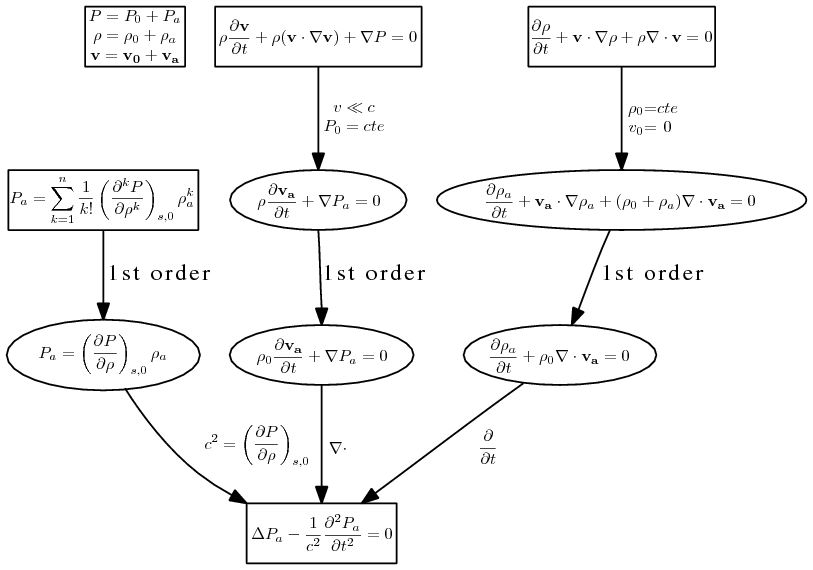
\includegraphics[width=0.6\textwidth]{figures/derivation_acoustic_wave_equation.png}
  NOTE: Important! Understand this diagram, will help to understand the meaning of the Euler equations!
  \item From the acoustic wave equation, one can derive the general solution for $\Delta \rho$ as a superposition of right-moving and left-moving waves:
  \begin{align}
    \Delta \rho(x,t) &= f_1(x-ct) + f_2(x+ct) \label{D'alambert rho} \\
    \Delta p(x,t) &= c^2 \Delta \rho(x,t) = c^2 [f_1(x-ct) + f_2(x+ct)] \\
    u(x,t) &= \frac{c}{\rho_0} [f_1(x-ct) - f_2(x+ct)] \label{D'alambert u}
  \end{align}
  EXPLANATION: After assuming the D'elambert solution for $\Delta \rho$, one can substitute it back into the system of equations to get a wave equation for $u$ (explanation about that at the botttom of pg. 8 in the book), and then substitute both into the systems of equations to get the relations:
  \begin{align}
    \Delta p &= c^2 \Delta \rho \\
    u &= \pm \frac{c}{\rho_0} \Delta \rho = \pm \frac{\Delta p}{\rho_0 c}
  \end{align}
  which is Eq. (1.33) in the book, The positive sign is for right-moving waves and the negative sign is for left-moving waves.
  \item \underline{Solving the D'alambert problem}: Given initial conditions $\Delta \rho(x,0) = g_1(x)$ and $u(x,0) = g_2(x)$, one can solve the system of equations defined by Eq. (\ref{D'alambert rho} and \ref{D'alambert u}) to get: 
  \begin{align}
    f_1 (x) + f_2 (x) &= g_1(x) \\ 
    f_1 (x) - f_2 (x) &= \frac{\rho_0}{c} g_2(x)
  \end{align}
  then one can solve for $f_1$ and $f_2$:
  \begin{align}
    f_1 (x) &= \frac{1}{2} \left[ g_1(x) + \frac{\rho_0}{c} g_2(x) \right] \\
    f_2 (x) &= \frac{1}{2} \left[ g_1(x) - \frac{\rho_0}{c} g_2(x) \right]
  \end{align}
  which is analogous to the Eq. at the top of pg. 9 in the book.
  \item At pg. 10 the book argues that wavelengths corresponsing to the frequencies audible to the human ear (20 Hz - 20 kHz) are $1.5 cm$ to $15 m$ (using $c \approx 330 m/s$), and the deviations of speed, density and pressure from their equilibrium values are very small, so the linearized equations are valid for sound waves in air.
\end{enumerate}

\subsection{Energy of perturbations}
\begin{enumerate}
  \item The energy density of the sound wave perturbations (per unit mass) is given by the first law of thermodynamics:
  \begin{align}
    d\varepsilon &= T dS - p dV \\
    &= -p dV \quad \text{(since $dS=0$ for adiabatic processes)} \\
    &= \frac{p}{\rho^2} d\rho \quad \text{(since $V=\frac{1}{\rho}$)}
  \end{align}
  so the isentropic derivatives of the specific energy is:
  \begin{align}
    \left(\frac{\partial \varepsilon}{\partial \rho}\right)_{S}&=\frac{p}{\rho^2}
    \\ \left(\frac{\partial^2 \varepsilon}{\partial \rho ^2}\right)_{S} &= \left( \frac{\partial}{\partial \rho} \left(\frac{p(\rho)}{\rho^2}\right) \right)_S = \frac{c^2}{\rho^2} -\frac{2p}{\rho^3}
  \end{align}
  
and the second-order change in energy for a perturbation of $\Delta \rho$ is:
  \begin{align}
    \varepsilon - \varepsilon_0 = &\left( \frac{\partial \varepsilon}{\partial \rho} \right)_{S,0} \Delta \rho + \frac{1}{2} \left( \frac{\partial^2 \varepsilon}{\partial \rho^2} \right)_{S,0} (\Delta \rho)^2 \\
    = &\frac{p_0}{\rho_0^2} \Delta \rho + \frac{1}{2} \left( \frac{c^2}{\rho_0^2} - \frac{2p_0}{\rho_0^3} \right) (\Delta \rho)^2
  \end{align}
  where the subscript $0$ indicates equilibrium values.
  The increment in energy per unit volume (here $\varepsilon$ is specific, i.e. per unit mass because we used $dV = \frac{1}{\rho^2} d\rho$) is  given by the disturbence in $\rho \varepsilon$:
  \begin{align}
    \rho \varepsilon - \rho_0 \varepsilon_0 &= \rho_0 \left( \varepsilon - \varepsilon_0 \right) + \varepsilon_0 \Delta \rho \\
    &= \rho_0 \left[ \frac{p_0}{\rho_0^2} \Delta \rho + \frac{1}{2} \left( \frac{c^2}{\rho_0^2} - \frac{2p_0}{\rho_0^3} \right) (\Delta \rho)^2 \right] + \varepsilon_0 \Delta \rho \\
    &= \left( \frac{p_0}{\rho_0} + \varepsilon_0 \right) \Delta \rho + \frac{1}{2} \left( \frac{c^2}{\rho_0} - \frac{2p_0}{\rho_0^2} \right) (\Delta \rho)^2 \\
    &= h_0 \Delta \rho + \frac{1}{2} \left( \frac{c^2}{\rho_0} - \frac{2p_0}{\rho_0^2} \right) (\Delta \rho)^2
  \end{align}
  where $h_0 = \varepsilon_0 + \frac{p_0}{\rho_0}$ is the specific enthalpy at equilibrium.
  Since $u = \frac{c}{\rho_0} \Delta \rho$, one term of the second-order energy increment can be written as:
  \begin{equation}
    \frac{1}{2} \rho_0 u^2 = \frac{1}{2} \rho_0 \left( \frac{c}{\rho_0} \Delta \rho \right)^2 = \frac{1}{2} \frac{c^2}{\rho_0} (\Delta \rho)^2
  \end{equation}
  so the total energy increment per unit volume, considering also the kinetic energy of the perturbation, is:
  \begin{equation}
    E - E_0 = h_0 \Delta \rho + \rho_0 u^2 - \frac{p_0}{\rho_0^2} (\Delta \rho)^2
  \end{equation}
  and \textcolor{red}{I have no idea how to neglect the term with $p_0$ in order to be able to say that} it is the same as Eq. (1.36) in the book.
  \textcolor{red}{Understand the example of wavepacket at the bottom of pg. 11 in the book!}
\end{enumerate}

\subsection{Problem of moving piston}
\begin{enumerate}
  \item This story has two cases - The piston moves at constant subsonic ($u << c$) speed in the period $0 < t < t_1$ and then stops - so a disturbence in density $\Delta \rho$ which is a rectangle in length $(c-u)t_1$ propagates to the right at speed $c$.
    \item The second case is that the piston moves at $-u$ at $t=t_1$ so two disturbences are created - one moving to the right and one to the left.
    \item \textcolor{red}{I asked chat GPT for why this is what happens, it said that a moving piston creates a continuous amount of delta waves as starting conditions, which creates a rectangle wave that moves at $c$ and its length is the integral over time of the piston movement, and obviously it moves at $c$}.
      \textbf{Figures 1.4 \& 1.5 in the book presents this well.}
      \item This problem is given as part of a discussion about cases where the energy of the perturbation has significant second-order terms in $\Delta \rho$.
\end{enumerate}
%%%%%%%%%%%%%%%%%%%%%%%%%%%%%%%%%%%%%%%%%%%%%%%%%%%%%%%%%%%%%%%%%%%%%%%%%%
\section{spherical Sound Waves}

\subsection{Deriving the acoustic wave equation}
\begin{enumerate}
    \item The linearized equations of mass and momentum conservation in spherical coordinates are given by:
    \begin{align}
      \frac{\partial \Delta \rho}{\partial t} + \frac{1}{r^2} \frac{\partial}{\partial r} (r^2 \rho_0 u) &= 0 \\
      \rho_0 \frac{\partial u}{\partial t} + \frac{\partial \Delta p}{\partial r} &= 0 \\
      \Delta p - c^2 \Delta \rho &= 0
    \end{align}
    \textcolor{red}{Understand the derivation of these equations from the general 3D Euler equations!}
    \item By defining new variables $\psi(r,t) = r u(r,t)$ and $\phi(r,t) = r \Delta \rho(r,t)$, one can rewrite the system of equations as:
    \begin{align}
      \frac{\partial \phi}{\partial t} + \rho_0 \frac{\partial \psi}{\partial r} &= 0 \\
      \rho_0 \frac{\partial \psi}{\partial t} + r \frac{\partial \Delta p}{\partial r} &= 0 \\
      \Delta p - c^2 \frac{\phi}{r} &= 0
    \end{align}
    \item By differentiating the first equation w.r.t time and substituting $\frac{\partial \psi}{\partial t}$ from the second equation into the differentiated first equation, one gets:
    \underline{Wave equation in spherical symmetry}:
    \begin{equation}
      \frac{\partial^2 \phi}{\partial t^2} - c^2 \frac{\partial^2 \phi}{\partial r^2} = 0
    \end{equation}
    and the solution is given by D'alambert's formula, when only outward-moving waves are considered:
    \begin{equation}
      \phi(r,t) = f(r-ct)
    \end{equation}
    which means that:
    \begin{equation}
      \Delta \rho(r,t) = \frac{f(r-ct)}{r}
    \end{equation}
    \item The book says that these spherical waves have amplitude that decreases as $\frac{1}{r}$ due to the geometric spreading of the wavefronts and using energy considerations ($\Delta\rho^2 r^2 \sim 1$ so $\Delta \rho \sim \frac{1}{r}$ in amplitude).
    \item Substituting $\Delta \rho$ into the momentum conservation equation, one can get the expression for the velocity perturbation $u(r,t)$:
    \begin{equation}
      u(r,t) = -\frac{c^2}{\rho_0}\left[\frac{f'(r-ct)}{r}-\frac{f(r-ct)}{r^2}\right]
    \end{equation}
    which is integrated over time to get Eq. (1.39) in the book:
    \begin{equation}
      u(r,t) = \frac{c}{\rho_0} \left[ \frac{f(r-ct)}{r} - \frac{\int^{r-ct}f(\xi)d\xi}{r^2} \right] = \frac{c}{\rho_0} \left[ \Delta \rho(r,t) - \frac{\varphi(r-ct)}{r^2}\right]
    \end{equation}
    where $\varphi(\eta) = \int^{\eta} f(\xi) d\xi$.
    \item The book discusses the fact that in order for the proportionality relation $\Delta u \sim \frac{c}{\rho_0} \Delta \rho$ to hold, we must satisfy $\varphi(r-ct) = 0$ which means that the total mass inside the spherical wave is zero (no net mass flow). This condition is satisfied only if the compression region ($\Delta \rho$ > 0) is followed by a rarefaction region ($\Delta \rho$ < 0) that happens at smaller $r$ values. This ensures that the total mass perturbation is zero, and this process is \textbf{Shown and Explained in Fig. 1.6 in the book}.
  \end{enumerate}
\section{Characteristics}
\begin{enumerate}
  \item Characteristics are curves in the space-time plane along which the partial differential equations (PDEs) governing fluid dynamics can be reduced to ordinary differential equations (ODEs). This simplification allows for easier analysis and solution of the equations.
  \item In section 3 it is shown that for 1D flow of an ideal compressible fluid, any arbitrary distrubence in velocity and pressure/density will cause the formation of a right and left moving wave, each propagating at speed $u \pm c$ respectively.
  \item One can claim that in the phase space of $(x,t)$, if a disturbence occurs at point $(x_0,t_0)$, then the disturbences will propagate along the characteristic lines defined by:
  \begin{align}
    C_+: \frac{dx}{dt} = u + c \label{char_plus} \\
    C_-: \frac{dx}{dt} = u - c \label{char_minus}
  \end{align}
  \underline{Difference between isentropic and adiabatic flow}: In an isentropic flow, the entropy remains constant along the flow and therefore the speed of sound $c$ has one degree of freedom. This can be shown using the definition of $c$ and the different relations for $p$ in isentropic and adiabatic flows:
  \begin{equation}
    c^2 = \left( \frac{\partial p}{\partial \rho} \right)_S
  \end{equation} 
  \begin{equation}
    p = K(S) \rho^\gamma \quad(\text{isentropic})
  \end{equation}
  \begin{equation}
    p = K \rho^\gamma \quad (\text{since } S=const)
  \end{equation}
  more detail about that in Eq. (\ref{p_of_S}) in this summary. Another place where it can be seen (chat GPT showed this) is by finding explicitly $dp(\rho, p)$ and showing that:
  \begin{align}
    dp = \left( \frac{\partial p}{\partial \rho} \right)_S d\rho + \left( \frac{\partial p}{\partial S} \right)_\rho dS \\
    dp = c^2 d\rho + P_S dS 
  \end{align}
  where $P_S = \left( \frac{\partial p}{\partial S} \right)_\rho = \frac{dK}{dS} \rho^\gamma = \frac{1}{C_V} K(s) = \frac{p}{C_V}$ and in summary:
  \begin{equation}
    dp = c^2 d\rho + \frac{p}{C_V} dS
  \end{equation}
  
  So here we clearly see that in non-isentropic flows ($dS \neq 0$), the pressure can vary due to both density and entropy changes, which is equivalent to two degrees of freedom for $c$.
  
  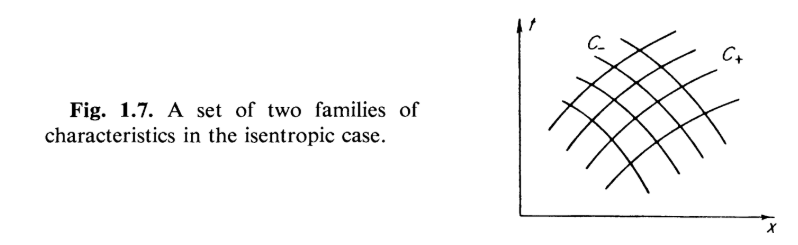
\includegraphics[width=1\textwidth]{figures/fig_1_7.png}
  
  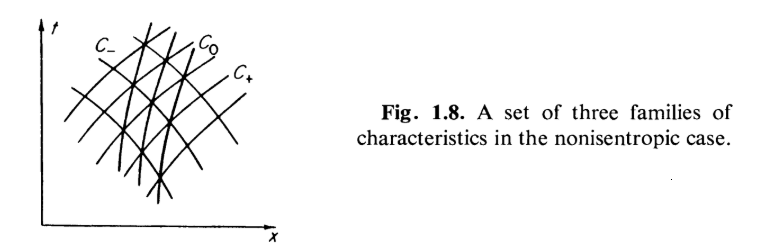
\includegraphics[width=1\textwidth]{figures/fig_1_8.png}
\end{enumerate}
\section{Plane isentropic flow \& Riemann invariants}
\begin{enumerate}
  \item In plane adiabatic flow, one can combine the acoustic equations to get the following relations along the characteristics:
  \begin{align}
    \left[ \frac{\partial u}{\partial t} + (u+c) \frac{\partial u}{\partial x} \right] + \frac{1}{\rho c} \left[ \frac{\partial p}{\partial t}+ (u + c) \frac{\partial p}{\partial x} \right] &= 0 \\
    \left[ \frac{\partial u}{\partial t} + (u-c) \frac{\partial u}{\partial x} \right] - \frac{1}{\rho c} \left[ \frac{\partial p}{\partial t}+ (u - c) \frac{\partial p}{\partial x} \right] &= 0
  \end{align}
  which means that:
  \begin{align}
    du + \frac{1}{\rho c} dp = 0 \quad \text{along } C_+ \\
    du - \frac{1}{\rho c} dp = 0 \quad \text{along } C_- \\
    dS = 0 \quad \text{along} C_0
  \end{align}
  In isentropic flow $dS=0$ everywhere, so the last equation is redundant. Then, the flow is \textbf{fully described using $u(x,t)$ and one of $\rho (x,t)$ or $p(x,t)$}, and the first two equations can be integrated to get the Riemann invariants:
  \begin{align}
    J_+ = u + \int \frac{dp}{\rho c} = const \quad \text{along } C_+ \\
    J_- = u - \int \frac{dp}{\rho c} = const \quad \text{along } C_-
  \end{align}
  derivations appear in pg. 18-19 in the book and more theoreticla explanation (using the generalized hodograph method) can be found in % insert link and show text instead of the link
  \href{https://en.wikipedia.org/wiki/Riemann_invariant#cite_ref-multiple_3-0}{Riemann invariant - Wikipedia} and specifically the example in there (which is exactly the derivation of the Riemann invariants for 1D isentropic flow):
  \begin{figure}[H]
    \centering
    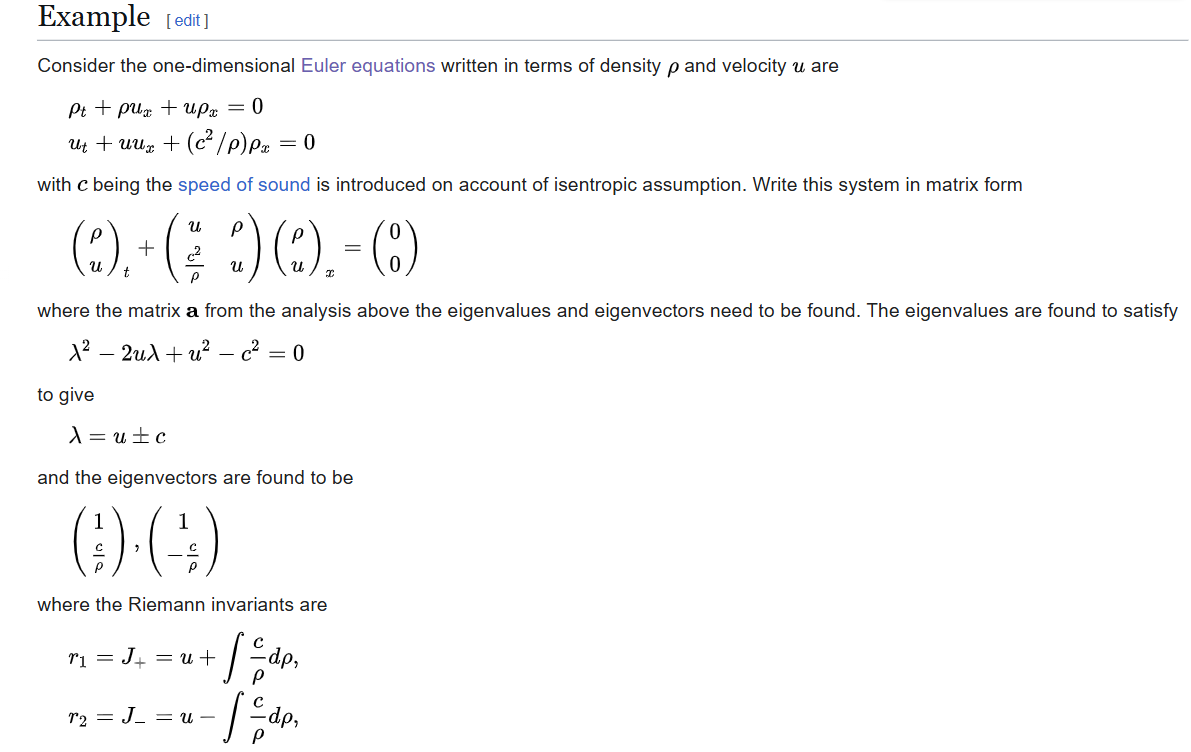
\includegraphics[width=1\textwidth]{figures/riemann_invariants_wikipedia.png}
    \caption{Riemann invariants derivation from Wikipedia}
  \end{figure}
  \item There is also a cool derivation in the bottom of pg. 20 that shows that for a slight perturbation from a constant state $(\rho_0, p_0, u_0)$, the Riemann invariants reduce to the linearized relations for right and left moving waves:
  \begin{align}
    J_+ &= u_0 + \Delta u + \int \frac{d\Delta p}{\rho c} \approx \Delta u + \frac{1}{\rho_0 c_0} \Delta p \\
    J_- &= u_0 + \Delta u - \int \frac{d\Delta p}{\rho c} \approx \Delta u - \frac{1}{\rho_0 c_0} \Delta p
  \end{align}
  and the equations of the characteristics $C_\pm$ reduce to:
  \begin{align}
    C_\pm: \frac{dx}{dt} = u_0 \pm c_0 \\
    \Rightarrow x - (u_0 \pm c_0) t = const
  \end{align}
  which means that the quantity $J_\pm$ (which is constant along $C_\pm$) is a function of $x - (u_0 \pm c_0) t$ only, so:
  \begin{align}
    \Delta u + \frac{1}{\rho_0 c_0} \Delta p &= f_1 (x - (u_0 + c_0) t) \\
    \Delta u - \frac{1}{\rho_0 c_0} \Delta p &= f_2 (x - (u_0 - c_0) t)
  \end{align}
  and adding/substructing the previous equations one gets:
  \begin{align}
    \Delta u &= f_1(x - (u_0 + c_0) t) + f_2(x - (u_0 - c_0) t) \nonumber \\
    \Delta p &= \rho_0 c_0 (f_1(x - (u_0 + c_0) t) - f_2(x - (u_0 - c_0) t))
  \end{align}
  
  and here we see again the \textbf{D'Alembert solution} for right and left moving waves in a moving fluid (with speed $u_0$).
\end{enumerate}

\subsection{Using invariants to describe the motion}
\begin{enumerate}
  \item The Riemann invariants can be used to describe the motion of a compressible fluid in 1D isentropic flow. More specifically, given full solution for $J_\pm (x,t)$ one can transform to:
  \begin{align}
    u(x,t) &= \frac{J_+ + J_-}{2} \\
    \int \frac{dp}{\rho c} &= \frac{J_+ - J_-}{2}
  \end{align}
  where in ideal gas with constant specific heats, the integral can be evaluated to get:
  \begin{equation}
    c = \frac{\gamma - 1}{4} (J_+ - J_-)
  \end{equation}
  Furthermore, knowing the full solution for $J_\pm (x,t)$ allows to find the characteristics $C_\pm$ by solving the ODEs:
  \begin{align}
    \frac{dx}{dt} = F_+ (J_+, J_-) \quad \text{along } C_+ \\
    \frac{dx}{dt} = F_- (J_+, J_-) \quad \text{along } C_-
  \end{align}
  where 
  \begin{align}
    F_+ (J_+, J_-) = u + c = \frac{\gamma + 1}{4} J_+ + \frac{3 - \gamma}{4} J_- \\
    F_- (J_+, J_-) = u - c = \frac{3 - \gamma}{4} J_+ + \frac{\gamma + 1}{4} J_-
  \end{align}
  \item These relations can help us \textbf{solve initial value problems}. Specifying the values of $J_\pm$ at initial points $A(x_1,0)$ and $B(x_2,0)$, one can trace the characteristics $C_+$ and $C_-$ from these points and find the values of $J_\pm$ or $u$ and $c$ at any point $(x,t)$ in the domain of dependence of $A$ and $B$. Specifically, knowing that $u_1,c_1$ are the values at point $A$ and $u_2,c_2$ are the values at point $B$, one can find $u(x,t)$ and $c(x,t)$ at the point of the cross of the characteristic $C_+$ from $A$ and $C_-$ from $B$ using:
  \begin{align}
    u(x,t) &= \frac{u_1 + u_2}{2} + \frac{c_1 - c_2}{\gamma - 1} \\
    c(x,t) &= \frac{c_1 + c_2}{2} + \frac{\gamma - 1}{2} (u_1 - u_2)
  \end{align}
  as described in pg. 22 in the book and shown in the figure below.
  
  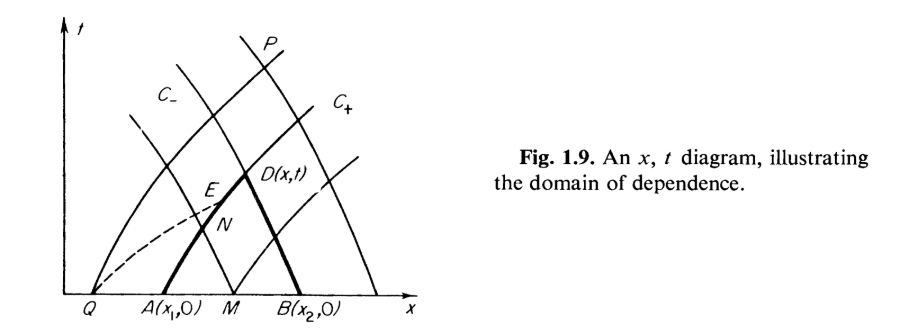
\includegraphics[width=1\textwidth]{figures/fig_1_9.png}
  
  NOTE: This method might seem a bit like a magic, but one should remember that \textbf{it works only after solving the characteristics ODEs} to find the point of intersection of $C_+$ and $C_-$.
\end{enumerate}

\subsection{Analyzing Causality}
\begin{enumerate}
  \item At the bottom of pg. 22 and pg. 23, it is explained that the solution at the point D at the previous figure depends only on the initial conditions between the points A and B (a slight change in the initial conditions at the point M affects the solution at D as well). However, a change in the initial conditions outside the interval AB doesn't affect the solution at D. 
  One can inverse the argument and say that the initial conditions along the segment AB affect only the solutions in the "region of influence" defined by the characteristics $C_-$ from A and $C_+$ from B, shown at the following figure.
  
  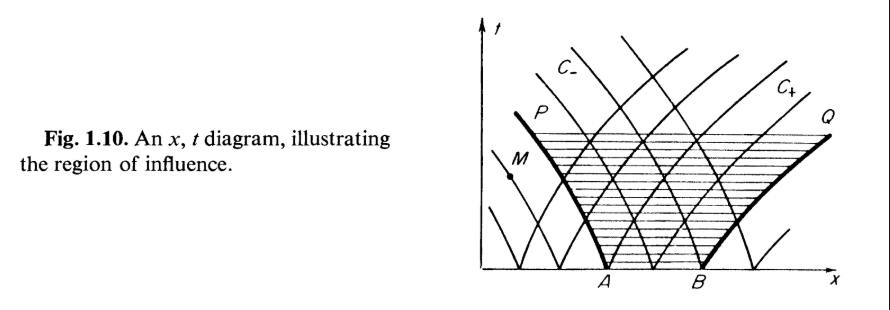
\includegraphics[width=1\textwidth]{figures/fig_1_10.png}
  \item At the top of pg. 24 it is described how one can approximate the solution at the point D by supposing that the characteristics outgoing from A and B are straight lines (constant speed). This approximation is valid for small times $t$ such that the change in speed along the characteristics is small. Using this approximation, one can find the coordinates of point D as:
  \begin{align}
    x_D &= x_1 + (u_1 + c_1) t \\
    x_D &= x_2 + (u_2 - c_2) t
  \end{align}
  which is actually what is done in the process of numeric solution of PDEs using the method of characteristics, and is fully described in figure 1.11 in the book.
  \end{enumerate}
\section{Plane isentropic gas flow in a bounded region}
\subsection{Causality and dependence on initial conditions}
\begin{enumerate}
  \item In a discussion from the bottom of pg. 24 until the top of pg. 26, the book shows that for a problem of a gas flow bounded by two moving pistons, knowing the initial conditions at $t=0$ and the motion of the pistons at the boundaries, one finds the solution at any point $(x,t)$ based on both the initial conditions of the flow at $t=0$ and the boundary conditions at the pistons (which are their functions of time). Elaboration on that is given in the book and shown in the figure below.
  
  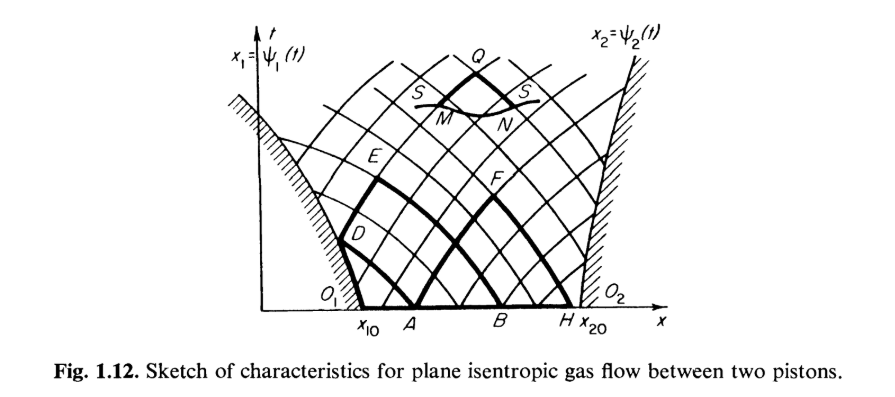
\includegraphics[width=1\textwidth]{figures/fig_1_12.png}
\end{enumerate}

\subsection{The physical meaning of the Riemann invariants}
\begin{enumerate}
  \item The book discusses (bottom of pg. 26 until the top of pg. 27) an experiment involving a flow bounded between 2 moving pistons, using a pressure gauge in order to calculate the Riemann invariants.
  The experiments involves placing a pressure gauge at a point $x$ between the pistons (at rest) in order to measure the pressure $p$ and therefore the invariants ($J_\pm = \cancel{u} \pm w(p) = \pm w(p_1)$ in the notation of the book) and then recalibrating \textcolor{red}{(Don't understand)} and measuring the pressure when the gauge is placed in parallel to the flow direction (\textcolor{red}{(for some reason that I don't understand)}) and then it then measures $w(p)$ and claims that this is the physical value and it is connected to the Riemann invariants by:
  \begin{equation}
    w(p) = \frac{1}{2} (J_+ - J_-)
  \end{equation}
  \end{enumerate}
  \section{Simple Waves}
  \begin{enumerate}
    \item Simple waves are isentropic flows where one of the Riemann invariants is constant throughout the flow field. For example, if $J_- = const$, then the flow is a simple wave characterized by $J_+$ or vice versa.
    \item For example, if $J_- = const$, then the defining equation for the characteristic $C_+$ is:
    \begin{equation}
      \frac{dx}{dt} = F_+ (J_+, J_-) = \frac{\gamma + 1}{4} J_+ + \frac{3 - \gamma}{4} J_-
    \end{equation}
    but since $J_-$ is constant and also \textbf{$J_+$ is constant along $C_+$} then $\frac{dx}{dt} = const$ along each characteristic $C_+$, which means that the characteristics are straight lines in the $(x,t)$ plane defined by the constant of $J_-$ and the value of $J_+$ along that characteristic (defined by an initial or boundary condition - boundary condition in case of flow bounded by pistons).:
    \begin{equation}
      x = F_+ (J_+, J_-) t + \varphi(J_+) \label{1.49}
    \end{equation}
    the book says that together with the equation $J_- = const$, these two equations fully define the flow field.
    \item Using the definition of $J_-$:
    \begin{equation}
      J_- = u - \int \frac{dp}{\rho c} = const 
    \end{equation}
    one can find the value for $c(u)$ (\textcolor{red}{I'm not sure where did $p$ go}) and then Eq. \ref{1.49} becomes:
    \begin{equation}
      x = \left[ u + c(u) \right] t + \varphi(u)
    \end{equation}
    or in other words, the solution is a right-travelling wave defined by the functional relation:
    \begin{align}
      u &= f \left( x - (u + c(u)) t \right) \\
      c &= g \left( x - (u + c(u)) t \right)
    \end{align}
    \textcolor{red}{I don't understand this part intuitively, what this right propagating wave means, how to imagine it and the fact that it has a nonlinear dispersion}.
    \item At the top of pg. 29, the book discusses the analogous case of a left travelling simple wave where $J_+ = const$ and the characteristics $C_-$ are straight lines in the $(x,t)$ plane.
  \end{enumerate}
\section{Distortion of simple waves and weak discontinuities}
\begin{enumerate}
  \item The bottom of pg. 29 says that the following discussion of non-linear phenomena in simple waves is somewhat an extension of the linear acoustic theory.
  \item First, the book (in the bottom of pg. 29) discusses the settings of the problem - supposing $J_- = const$ (globally) and initial profiles of $u(x,0)$ and $c(x,0)$ at $t=0$ shown in fig. 1.13a in the book.
  
  These are then propagated to the right using the characteristics $C_+$ which are straight lines \textbf{with different slopes of $u+c(u)$ determined by the initial profiles of $u(x)$ and $c(x)$} in the $(x,t)$ plane. The characteristics $C_+$ are shown in fig. 1.13b and the propagated simple wave at time $t_1$ is shown in fig. 1.13c.
  
  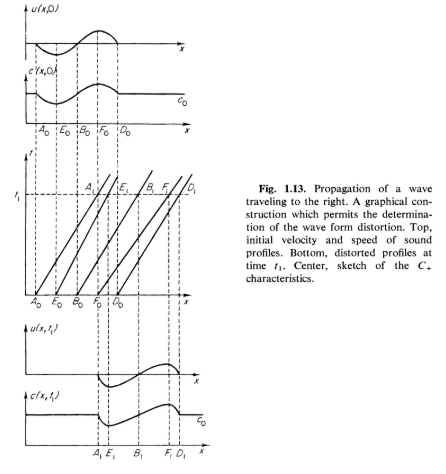
\includegraphics[width=1\textwidth]{figures/fig_1_13.png}
  \item The book then discusses the fact that since the characteristics $C_+$ have different slopes (speeds) determined by the initial profiles of $u(x)$ and $c(x)$, then after some time $t=t_3$, two characteristics will \textbf{intersect} at a point in the $(x,t_3)$.
  
  This causes an apparent "overshoot" in the profile of $u(x,t_3)$ and $c(x,t_3)$ shown in fig. 1.14d and is solved using the interpretation of weak discontinuity shown in fig 1.14e.
  
  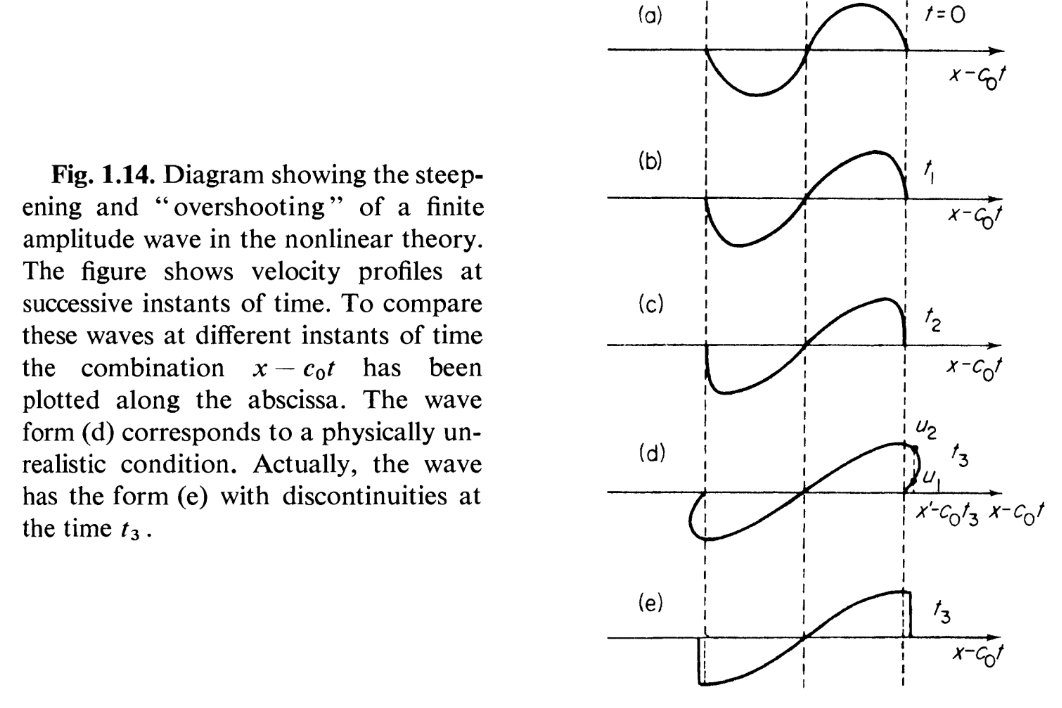
\includegraphics[width=1\textwidth]{figures/fig_1_14.png}
  \item A discussion about the interpretation of the weak discontinuity is given in the top of pg. 32, and is illustrated in fig. 1.15.
  
  This interprets it as a small disturbance that has to propagate at the speed of sound (\textcolor{red}{I don't understand this part well}).
  
  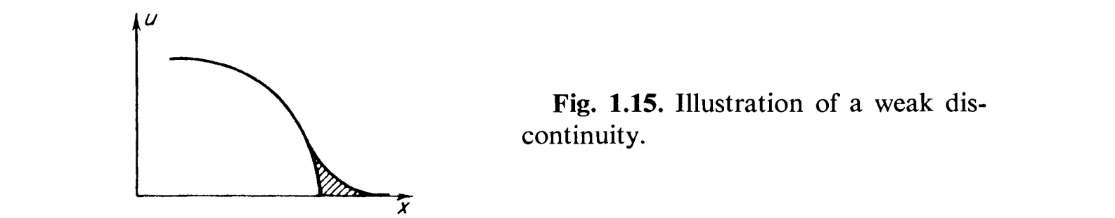
\includegraphics[width=1\textwidth]{figures/fig_1_15.png}
  
  Then fig. 1.16 illustrates the statement "If the isentropic flow has a common boundary with a region of uniform flow, then this flow is necessarily a simple wave".
  
  The explanation is that since the uniform flow has constant $J_+$ and $J_-$, then at the boundary with the isentropic flow, one of the Riemann invariants must be constant (\textcolor{red}{because of continuity?}).
  
  This means that the isentropic flow is a simple wave. Illustration is shown in fig. 1.16.
  
  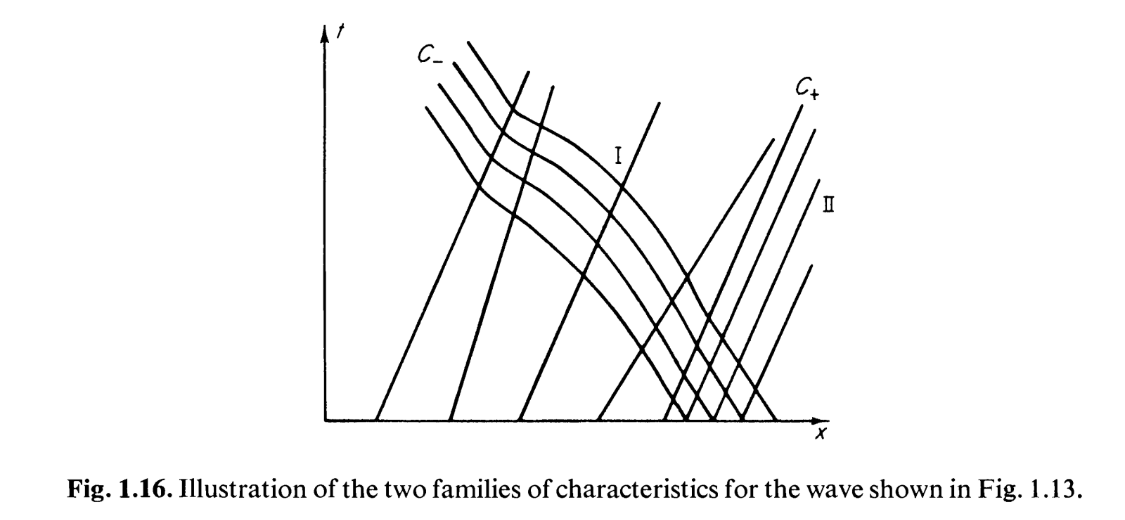
\includegraphics[width=1\textwidth]{figures/fig_1_16.png}
\end{enumerate}
\section{The rarefaction wave}
\subsection{Finding the Simple wave solution for the rarefaction wave}
\begin{enumerate}
  \item \textcolor{red}{"As shown in the proceding section, the motion of gas initially with a constant velocity and pressure (i.e. constant Riemann invariants) adjacent to a piston that is suddenly set into motion away from the gas, \textbf{results in the formation of a simple wave called a rarefaction wave.}"} \textcolor{blue}{I must understand it through the explanation appearing at the introduction of section 1.8 which is in pg. 27}.
  \item The book presents a problem of a piston at $x=0$  that slowly accelarates backwards (to the left) from rest at $t=0$ into velocity of $-U$ at time $t=t_1$. Stating that the gas is initially at rest with pressure $p_0$ and density $\rho_0$, one can find the solution for the flow using the Riemann invariants and the simple wave theory!
  \item For an ideal gas with constant specific heats (though this solution can be extended to more general thermodynamic properties of the gas if the integral in the Riemann invariants can be evaluated), the Riemann invariant $J_-$ which is constant throughout the flow field is:
  \begin{equation}
    J_- = u - \frac{2c}{\gamma - 1} = - \frac{2 c_0}{\gamma - 1} \quad \Rightarrow \quad \boxed{c(u) = c_0 + \frac{\gamma - 1}{2} u}
  \end{equation}
  \item Once $c(u)$ is known, we know from section 1.8 about simple waves that the characteristics $C_+$ are defined by the following equations (straight lines with slope $u+c(u)$):
  \begin{equation}
    \boxed{\left(\frac{dx}{dt}\right)_{C_+}} = u + c(u) = u + c_0 + \frac{\gamma - 1}{2} u = c_0 + \frac{\gamma + 1}{2} u = \boxed{c_0 - \frac{\gamma + 1}{2} |\omega|}
  \end{equation}
  where $\omega = -u$ is the speed of the piston (positive value).
  In order to achieve a full solution, one should just find the functional relation between $u$ and $x$ and $t$ using the boundary condition at the piston! For that \textbf{an explicit functional form of the piston motion $U(t)$ is needed.} 

  The formula for the characteristics $C_+$ sheds light on the geometric structure of the characteristics in the $(x,t)$ plane and the profile of $u(x)$ and $c(x)$ which change smoothly between different times. An analysis and discussion about this is given in pg. 34-35 in the book along with fig. 1.17 and fig. 1.18.
  
  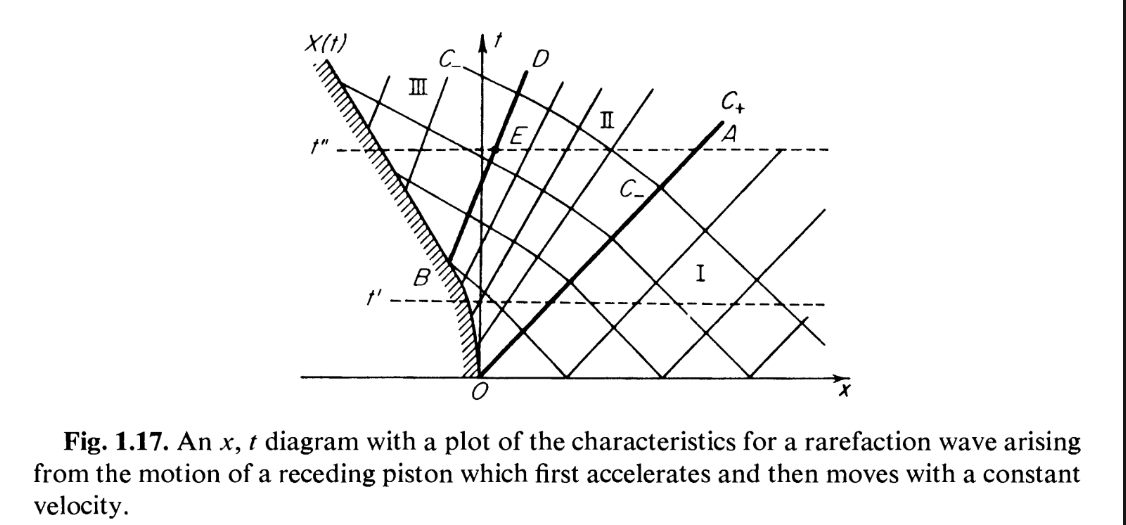
\includegraphics[width=1\textwidth]{figures/fig_1_17.png}
  
  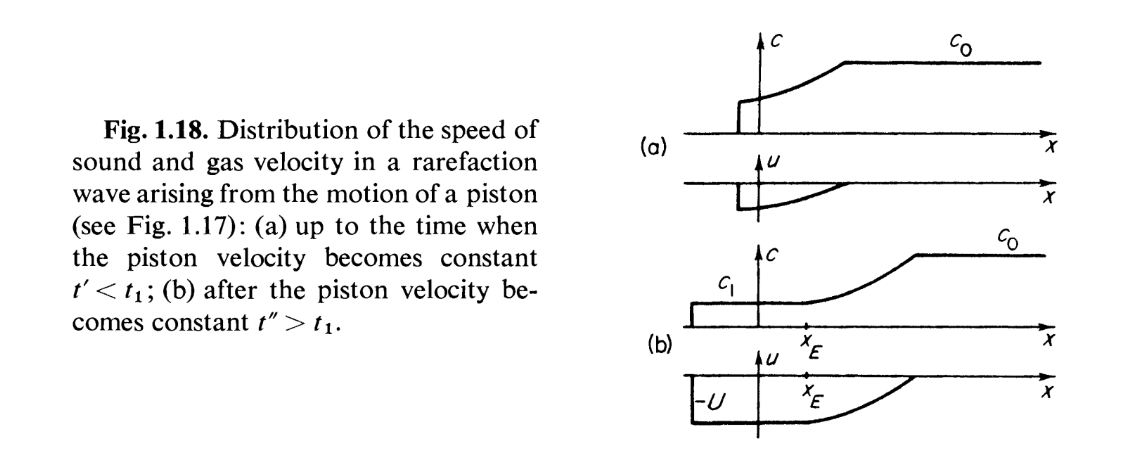
\includegraphics[width=1\textwidth]{figures/fig_1_18.png}
\end{enumerate}

\subsection{An example for a specific \texorpdfstring{$w(t)$}{w(t)}}
\begin{enumerate}
  \item The book gives an example for a specific piston motion:
  \begin{equation}
    w(t) = -U(1 - e^{-t/\tau}) \quad \tau > 0
  \end{equation}
  where $U$ is the final speed of the piston and $\tau$ is a characteristic time of the piston acceleration.
  \item integrating over time, one gets the position of the piston as:
  \begin{equation}
    X(t) = -Ut + U \tau (1 - e^{-t/\tau})
  \end{equation}
  which approaches the straight line $X(t) = -U(t-\tau)$ as $t >> \tau$, which is a valid boundary condition for the piston motion, that can be used to find the function $\varphi(u)$ needed to find the full solution for $u(x,t)$ and $c(x,t)$!
  \begin{equation}
    X(t) = \left[ c_0 - \frac{\gamma + 1}{2} |w(t)| \right] t + \varphi (|w(t)|)
  \end{equation}
  substituting the assymptotic expression for $X(t)$, one gets the velocity distribution with respect to $x$ in the implicit form:
  \begin{equation}
    \boxed{x = \left[ c_0 + \frac{\gamma + 1}{2} u \right] t - u\tau + \tau(c_0 + \frac{\gamma + 1}{2} u + U) \ln \left( 1 + \frac{u}{U} \right)}
  \end{equation}
  which is valid according to the book in the region $X(t) < x < c_0 t$ and \textcolor{red}{didn't understand why it isn't the smaller region $-U(t-\tau) < x < c_0 t$.}
  \item The book also discusses the case of a "central rarefaction wave" where the piston accelarates instantaneously and the characteristic lines BD and OC in fig 1.17 intersect at the origin, which makes the solution of $u(x,t)$ be linear in $x$ as shown in Eq. 56 in the book, since the $\varphi(u) = 0$ in that case (it can be shown by substituting $X(t) = -Ut$ into the general formula for $X(t)$ above):
  \begin{equation}
    |u|(x,t) = \frac{2}{\gamma + 1} \left( c_0 - \frac{x}{t} \right) \quad \text{for } -Ut < x < c_0 t
  \end{equation} 
  \item \textcolor{green}{The bottom of pg. 37 includes an explanation for the expressions for $p$ and $\rho$ in the centered rarefaction wave, using the isentropic relations for an ideal gas with constant specific heats. I understood them but didn't write them here because of time contraints.}
\end{enumerate}
\section{Self similarity in the rarefaction wave}
\begin{enumerate}
  \item The book discusses (pg. 37 bottom - pg. 38) the fact that the expressions for the centered rarefaction wave depend only on the variable $\xi = \frac{x}{t}$, and relate it to the fact that this problem has no intrinsic length or time scales except velocity scales like $c_0$ and $U$. \item One can write the Euler equations in terms of $\xi=\frac{x}{t}$ and find ODEs for $u(\xi)$ and $c(\xi)$ which can be solved to get...
\end{enumerate}

\subsection{Self-similaritty solution}
\begin{enumerate}
  \item \underline{Finding the partial derivatives in terms of $\xi$}:
  For every function $f(x,t)$ the following relations hold:
  \begin{align}
    \frac{\partial f}{\partial t} &= \frac{df}{d\xi} \frac{\partial \xi}{\partial t} = \frac{df}{d\xi} \left( -\frac{x}{t^2} \right) = -\frac{\xi}{t} \frac{df}{d\xi} \\
    \frac{\partial f}{\partial x} &= \frac{df}{d\xi} \frac{\partial \xi}{\partial x} = \frac{df}{d\xi} \left( \frac{1}{t} \right) = \frac{1}{t} \frac{df}{d\xi}
    \frac{Df}{Dt} = \frac{\partial f}{\partial t} + u \frac{\partial f}{\partial x} = \frac{1}{t} (u - \xi) \frac{df}{d\xi}
  \end{align}
  \item \underline{Finding the Euler equations in terms of $\xi$}:
  \begin{align}
    \frac{D\rho}{Dt}=-\rho \frac{\partial u}{\partial x} &\Rightarrow (u - \xi) \frac{d\rho}{d\xi} + \rho \frac{du}{d\xi} = 0 \\
    \rho \frac{Du}{Dt} = -\frac{\partial p}{\partial x} &\Rightarrow \rho (u - \xi) \frac{du}{d\xi} + \frac{dp}{d\xi} = 0 \\
    \rho T \frac{DS}{Dt} = 0 &\Rightarrow (u - \xi) \frac{dS}{d\xi} = 0
  \end{align}
  \item and now the real magic happens. If we neglect the trivial solution of $u=\xi$ (hence constant fields and a uniform flow), then from the last equation we get that $S=const$ (isentropic flow) and therefore we can use the isentropic relation for $dp$ to get:
  \begin{equation}
    dp = c^2 d\rho \Rightarrow \frac{dp}{d\xi} = c^2 \frac{d\rho}{d\xi}
  \end{equation}
  and then substituting the second equation into the first one to eliminate $\frac{d\rho}{d\xi}$, we get:
  \begin{equation}
    \left[ (u - \xi)^2 - c^2 \right] \frac{d\rho}{d\xi} = 0
  \end{equation}
  which means that $u-\xi = \pm c$ and so $\xi = u \pm c$.
  Substituting this relation inside the first equation, one gets:
  \begin{equation}
    \pm c \frac{\partial \rho}{\partial \xi} + \rho \frac{\partial u}{\partial \xi} = 0
  \end{equation}
  which can be rearranged to:
  \begin{equation}
    du \pm \frac{1}{\rho c} dp = 0
  \end{equation}
  which are exactly $dJ_{\pm} = 0$!!! 
\end{enumerate}

\subsection{Analyzing the affect of the rarefaction wave over a single particle}
\begin{enumerate}
  \item The path of each particle in the rarefaction wave can be found by solving the ODE (with some initial condition $x_0$ at $t_0$):
  \begin{equation}
    \frac{dx}{dt} = u(x,t)
  \end{equation}
  which essentially means integrating over the velocity field $u(x,t) = \frac{2}{\gamma - 1} \left( c_0 - \frac{x}{t} \right)$.
  Since the right-moving wave propagates in the speed of $c_0$, one should notice that a particle initially at position $x_0$ will be affected by the wave only after time $t_0 = \frac{x_0}{c_0}$. This claim is illustrated in fig. 1.21 in the book.
  
  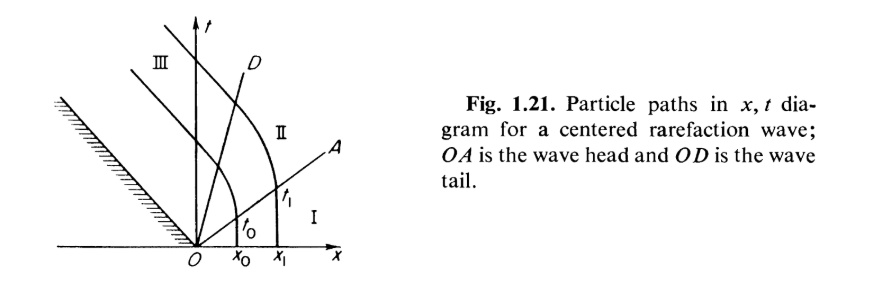
\includegraphics[width=1\textwidth]{figures/fig_1_21.png}
  \item It is also claimed that the faster the piston moves (larger $|U|$), the lower are $c$, $p$ and $\rho$ in the rarefaction wave (Eq. 1.53-1.56 in the book), which can be seen from the expressions for $c$, $p$ and $\rho$ (that all include negative expressions of $|U|$), and therefore there is a limit for the piston speed $|U| < \frac{2 c_0}{\gamma - 1}$ in order to keep $c$, $p$ and $\rho$ positive in the rarefaction wave.
  \item However, there is a CAVEAT that says that physically, the piston speed can exceed that limit and thereby create a vacuum region in the gas. The particles will accelarate to the assymptotic speed of $|u|_{max} = \frac{2 c_0}{\gamma - 1}$ and the density and pressure will approach zero. This phenomenon is explained in pg. 42 in the book along with fig. 1.22.
  
  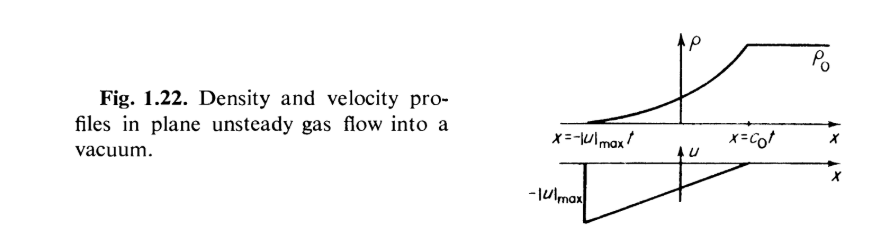
\includegraphics[width=1\textwidth]{figures/fig_1_22.png}  
  \textcolor{red}{I still need to make sure that I know how  to derive these profiles from the equations}.
\end{enumerate}

\subsection{Analyzing the vaccum solutio using Bernoullie's equation}
\begin{enumerate}
  \item The book discusses (pg. 42-43) the use of Bernoullie's equation in order to analyze the vacuum solution, where it uses the steady flow Bernoullie's equation along a streamline from the undisturbed gas to the point where the vacuum is formed.
  \textcolor{red}{I didn't have time to write this part, it involves studying the Bernoullie's equation}.
\end{enumerate}
\section{On the impossibility of the existence of a centered compression simple wave}
\begin{enumerate}
  \item The book discusses (pg. 43-44) the fact that a centered compression simple wave (the opposite of a rarefaction wave) is impossible, since it will require its tail to move faster than its head, which creates a graph that is opposite to fig 1.20 (the velocity profile of a centered rarefaction wave) and is actually non-physical.
  \item \textcolor{red}{I neglected here the full understanding of the calculation appearing in pg. 43 of the velocity profile}. The figures are shown in the book.
\end{enumerate}
\section{Gas dynamics of shock waves}
\subsection{Problem setting and conservation equations}
\begin{enumerate}
  \item \underline{Mathematical background:} In section 11 we showed that \textbf{since the problem is self-similar, the only solutions that satisfy the Euler equations are trivial uniform flows or centered simple waves}. However, in section 12 we showed that \textbf{a centered compression simple wave is *impossible*}.
  
  Therefore, the only solution eliminates the unreal region II in fig 1.19 and creates a discontinuity (shock wave) between regions I and III. 
  
  \item \underline{initial gas parameters}: The gas is initially at rest ($u=0$) with uniform pressure $p_0$ and density $\rho_0$.
  \item \underline{shock wave parameters}: The piston moves at velocity $u_1$ (causing the particles trapped in the shock region to have the same velocity) and the shock wave moves to the right with speed $D$.
  
  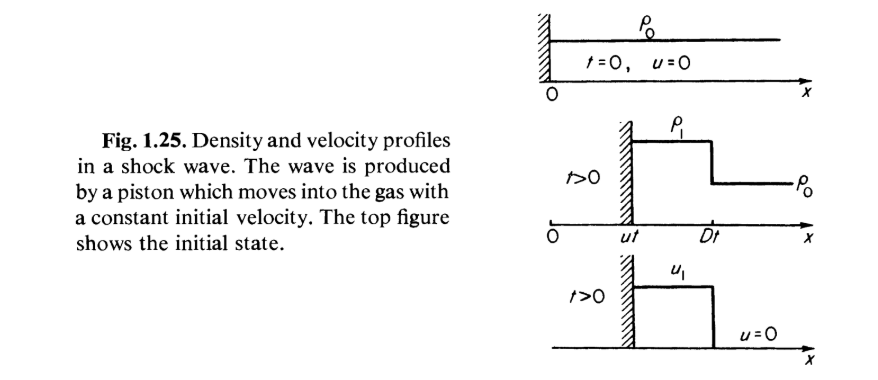
\includegraphics[width=1\textwidth]{figures/fig_1_25.png} 
  \item \underline{Conservation equations across the shock}: The conservation equations across the shock (in the lab frame of reference) are: \newline
  \underline{Mass conservation}: \newline
  At time $t$, the mass (per unit of one cross section) of the gas that already entered the shock region (looking at the top profile in Fig 1.25) is $\rho_0 D t$. The mass of the gas that is actually inside the shock region (according to the lower figures in Fig 1.25) at time $t$ is $\rho_1 (D - u) t$.
  \begin{equation}
    \rho_0 D t = \rho_1 (D - u_1) 
  \end{equation}
  \underline{Momentum conservation}: \newline
  THe total momentum of the gas at the shock region at time $t$ is Mass $\times$ velocity = $\rho_0 D t \cdot u$ (according to the Mass conservation equation). The change in momentum is caused by the net pressure (which is force per unit area of one cross section) acting over time $t$:
  \begin{equation}
    \rho_0 D t = (p_1 - p_0)t 
  \end{equation}
  Note that the pressure $p_1$ is the pressure that the gas in the shock region exerts on the environment (to the right).

  \underline{Energy conservation}: \newline
  Here the argument says that the change in the total energy of the gas in the shock region at time $t$ is Mass $\times$ (change in internal energy + kinetic energy) = $\rho_0 D t \left( \varepsilon_1 + \frac{u^2}{2} \right)$. This should be equal to the work done by the gas at pressure region over time $t$ which is $p_1 u t$.
  
  \begin{equation}
    \rho_0 D t\left(\varepsilon_1 - \varepsilon_0 + \frac{u^2}{2}\right) = p_1 u t 
  \end{equation}
\end{enumerate}

\subsection{Changing to the shock frame of reference}
\begin{enumerate}
  \item It is often more convenient to analyze the shock wave in the shock frame of reference, where the shock is stationary and the \textbf{gas flows into the shock at speed $u_0 = -D$} from the right and \textbf{exits the shock at speed $u_1=-(D-u)$} to the left.
  \item Thus, the conservation equations in the shock frame of reference are:
  \begin{align}
    \text{Mass conservation:} &\quad \rho_0 u_0 = \rho_1 u_1 \\
    \text{Momentum conservation:} &\quad p_0 + \rho_0 u_0^2 = p_1 + \rho_1 u_1^2 \\
    \text{Energy conservation:} &\quad \varepsilon_0 + \frac{p_0}{\rho_0} + \frac{u_0^2}{2} = \varepsilon_1 + \frac{p_1}{\rho_1} + \frac{u_1^2}{2}
  \end{align}
  there is also a reference to the Bernoullie's equation for steady flow along a streamline, which is essentially the same as the energy conservation equation above:
  \begin{equation}
    h + \frac{u^2}{2} = \varepsilon + \frac{u^2}{2} + \frac{p}{\rho} = const
  \end{equation}
  \item \underline{Derivation of the conservation equations}: \newline
  These equations can actually be achieved through integrating over the Euler equations in their "Flux" form (the flux for mass, momentum and energy) across the shock discontinuity. This is shown through Eqs. (1.65) in the book:
  \begin{align}
    \frac{\partial \rho}{\partial t} &= -\frac{\partial}{\partial x}  (\rho u)  \\
    \frac{\partial (\rho u)}{\partial t} &= -\frac{\partial }{\partial x} (p + \rho u^2)\\
    \frac{\partial}{\partial t} \left( \rho \varepsilon + \frac{1}{2} \rho u^2 \right) &= -\frac{\partial}{\partial x} \left[ \rho u \left(  \varepsilon + \frac{1}{2}  u^2 + \frac{p}{\rho} \right) \right]
  \end{align}
\end{enumerate}
\section{Huguniot Curves}
\begin{enumerate}
  \subsection{The derivation of the Huguniot Curve}
  \item First, one should rearrange the mass equation through the definition of the specific volume $V = \frac{1}{\rho}$ to get:
  \begin{equation}
    \frac{V_0}{V_1} = \frac{u_0}{u_1}
  \end{equation}
  Then, eliminating $u_0$ and $u_1$ from the momentum equation using the mass equation (with the specific volume), one gets:
  \begin{align}
    u_0^2 &= V_0^2 \frac{p_1 - p_0}{V_0 - V_1} \\
    u_1^2 &= V_1^2 \frac{p_1 - p_0}{V_0 - V_1} \label{u_shock}
  \end{align}
  Substituting this relations into the energy equation, one gets the Huguniot equation:
  \begin{equation}
    \varepsilon_1 - \varepsilon_0 = \frac{1}{2}(p_1 + p_0) (V_0 - V_1) \label{Hugoniot Energy}
  \end{equation}
  which is often denoted using the enthalpy $h = \varepsilon + pV$ as:
  \begin{equation}
    h_1 - h_0 = \frac{1}{2} (p_1 - p_0)(V_0 + V_1) \label{Hugoniot}
  \end{equation}
  which in general can be written as:
  \begin{equation}
    p_1 = H(V_1; p_0, V_0)
  \end{equation}
  \item The Huguniot equation describes the possible end states $(p_1, V_1)$ that can be achieved through a shock wave from a given initial state $(p_0, V_0)$.
  \item In that manner, it is analogous to the isentropic relations that describe the possible end states that can be achieved through isentropic processes from a given initial state throgh the isentropic relation $p_1=P(V_0,S)$. However, the set of possible isentropic curves is parametered using 1D parameter $S$ (entropy), while the Huguniot curves are parametered using 2D parameters $(p_0, V_0)$.
\end{enumerate}
\section{Shock waves in an ideal gas with constant specific heats}
\subsection{Analyzing the Huguniot curves}
\begin{enumerate}
  \item The internal energy and enthalpy for an ideal gas with constant specific heats are:
  \begin{align}
    \varepsilon &= c_v T = \frac{p V}{\gamma - 1} \\
    h =& c_p T = \frac{\gamma p V}{\gamma - 1}
  \end{align}
  and therefore they can be directly substituted into the Huguniot equation (Eq. \ref{Hugoniot}) to get:
  \begin{equation}
    \frac{\gamma}{\gamma - 1} (p_1 V_1 - p_0 V_0) = \frac{1}{2} (p_1 - p_0)(V_0 + V_1)
  \end{equation}
  which can be rearranged to:
  \begin{equation}
    \frac{p_1}{p_0} = \frac{(\gamma + 1)V_0 - (\gamma - 1)V_1}{(\gamma + 1)V_1 - (\gamma - 1)V_0} \label{Hugoniot_ideal_gas}
  \end{equation}
  \item For some reason (that the book says will become clear at section 1.17), the book calims that the Huguniot curve is physically unattainable for $V_1 > V_0$ (expansion shock) and shows it as a dashed line in fig. 1.27
  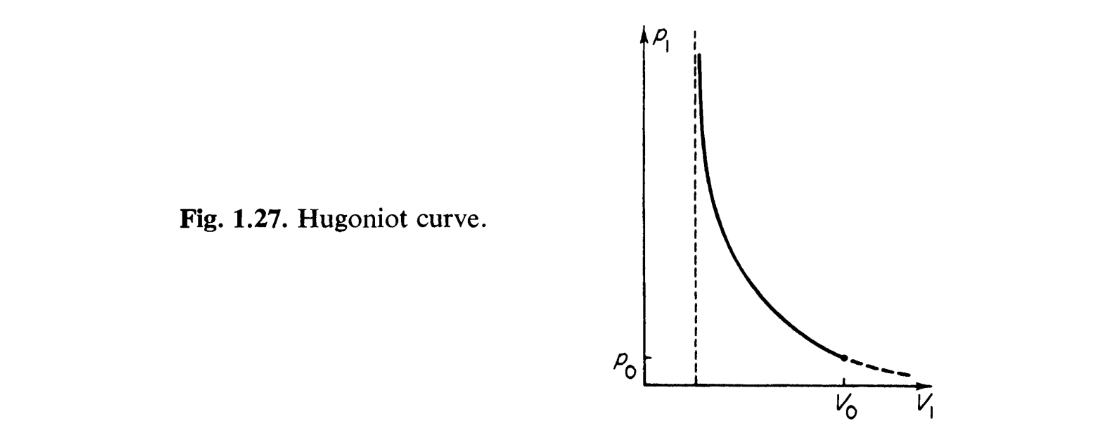
\includegraphics[width=1\textwidth]{figures/fig_1_27.png}
  \item The book also considers the ratio of densities or specific heats (they are inversely proportional) that are easily produced from the Hugoniot equation (Eq. \ref{Hugoniot_ideal_gas}):
  \begin{equation}
    \frac{\rho_1}{\rho_0} = \frac{V_0}{V_1} = \frac{(\gamma + 1)p_1 + (\gamma - 1)p_0}{(\gamma - 1)p_1 + (\gamma + 1)p_0}
  \end{equation}
  Even if $p_1 \gg p_0$, the density ratio is bounded by:
  \begin{equation}
    \frac{\rho_1}{\rho_0} < \frac{\gamma + 1}{\gamma - 1}
  \end{equation}
  and the book discusses that in monoatomic ideal gas this ratio equals 4, in diatomic ideal gas it equals 6 and even at gases with high temperatures, vibrational modes, ionization and variating specific heats, this ratio is still bounded and cannot exceed 11-13.
\end{enumerate}
\subsection{Limits of strong \& weak shocks}
\begin{enumerate}
  \item As we have seen, the density ratio across the shock is bounded. When $p_1 \gg p_0$ and $\frac{V_1}{V_0} \approx \frac{\gamma - 1}{\gamma + 1}$, the increase in temperature is proportional to the pressure increase:
  \begin{equation}
    \frac{T_1}{T_0} = \frac{p_1 V_1}{p_0 V_0} \approx \frac{(\gamma - 1)}{(\gamma + 1)} \frac{p_1}{p_0}
  \end{equation} 
  \item The equations for the ratio $\frac{V_0}{V_1}$ and the equations for the velocities \ref{u_shock} can be rearranged to get:
  \begin{align}
    u_0^2 &= \frac{V_0}{2} \left[(\gamma - 1)p_0 + (\gamma + 1)p_1 \right] \\
    u_1^2 &= \frac{V_0}{2} \frac{\left[(\gamma + 1)p_0 + (\gamma - 1)p_1 \right]^2}{\left[ (\gamma - 1)p_0 + (\gamma + 1) p_1 \right]^2}
  \end{align}
  which in the limit of strong shocks ($p_1 \gg p_0$) become:
  \begin{align}
    u_0^2 &\approx \frac{(\gamma + 1)}{2} p_1 V_0 \\
    u_1^2 &\approx \frac{(\gamma - 1)^2}{2(\gamma + 1)} p_1 V_0
  \end{align}
  knowing that the speed of sound in the gas is:
  \begin{equation}
    c_{0,1}^2 = \gamma p_{0,1} V_{0,1}
  \end{equation}
  one can write the Mach numbers of the flow into and out of the shock as:
  \begin{align}
    M_0^2 &= \frac{u_0^2}{c_0^2} \approx \frac{(\gamma + 1)}{2\gamma} \frac{p_1}{p_0} \\
    M_1^2 &= \frac{u_1^2}{c_1^2} \approx \frac{(\gamma - 1)}{2\gamma}
  \end{align}
  which are exactly Eq. (1.83) and (1.84) in the book under the limit $p_1 \gg p_0$.\
  \item In a discussion at the top of pg. 53 in the book, it claims that in the limit of weak shocks ($p_1 \approx p_0$), Eq. (1.83) and (1.84) still hold (\textcolor{red}{which I don't understand, because they assumed Eq. (1.82) that assumes $p_1 \gg p_0$}) the Mach number become close to unity (i.e. $u_0 \approx c_0 \approx c_1 \approx u_1$) and the shock wave becomes a weak discontinuity that can be analyzed using the linear acoustic theory (since the perturbations in pressure, density and velocity are small).
  \item Physically speaking, the gas enters the shock region at supersonic speed ($M_0 > 1$) and exits the shock region at subsonic speed ($M_1 < 1$). The Mach number of the supersonic flow into the shock can be arbitrarily large (strong shock) while the Mach number of the subsonic flow ($M_0 \to \infty$) out of the shock is bounded by $M_1 \geq \sqrt{\frac{\gamma - 1}{2\gamma}}$ which is less than 1 for every $\gamma > 1$.
\end{enumerate}
\subsection{Increase in Entropy}
\begin{enumerate}
  \item The book discusses (pg. 53 bottom - 54) the fact that the entropy increases across the shock wave according to the formula:
  \begin{equation}
  \begin{aligned}
    S_1 - S_0 &= c_v \ln \left[ \frac{p_1}{p_0} \left( \frac{V_1}{V_0} \right)^{\gamma} \right] \\
    &= c_v \ln \left[ \frac{(\gamma + 1)p_1 + (\gamma - 1)p_0}{(\gamma - 1)p_1 + (\gamma + 1)p_0} \left( \frac{(\gamma + 1)V_0 - (\gamma - 1)V_1}{(\gamma + 1)V_1 - (\gamma - 1)V_0} \right)^{\gamma} \right]
  \end{aligned}
  \end{equation} 
  from which one can see that for weak shocks ($p_1 \approx p_0$), the entropy increase is very small (second order in the pressure difference), and for strong shocks ($p_1 \gg p_0$), the entropy increase is large and proportional to $\ln(p_1/p_0)$, which is unbounded.\
  \item The book says that the increase in entropy happens due to the irreversible nature of the shock wave, and is derived from the conservation laws.
  It says that \textbf{the rate of the increase in entropy} is not determined by the Euler equations, but rather by the \textbf{dissipative processes} (like viscosity and heat conduction) that rely on length scales which are the mulecular mean free path that is neglected in the discussion of the Euler equations.
\end{enumerate}
\section{Geometric interpretation of the shock relations}
\subsection{The relation between the Hugoniot and Isentrope curves}
\begin{enumerate}
  \item Suppose a gas initially at state $A(p_0, V_0)$. This state defines the curve of possible end states that can be achieved through isentropic processes (the isentrope curve) and the curve of possible end states that can be achieved through shock waves (the Hugoniot curve), shown in Fig. 1.28.
  \begin{center}
      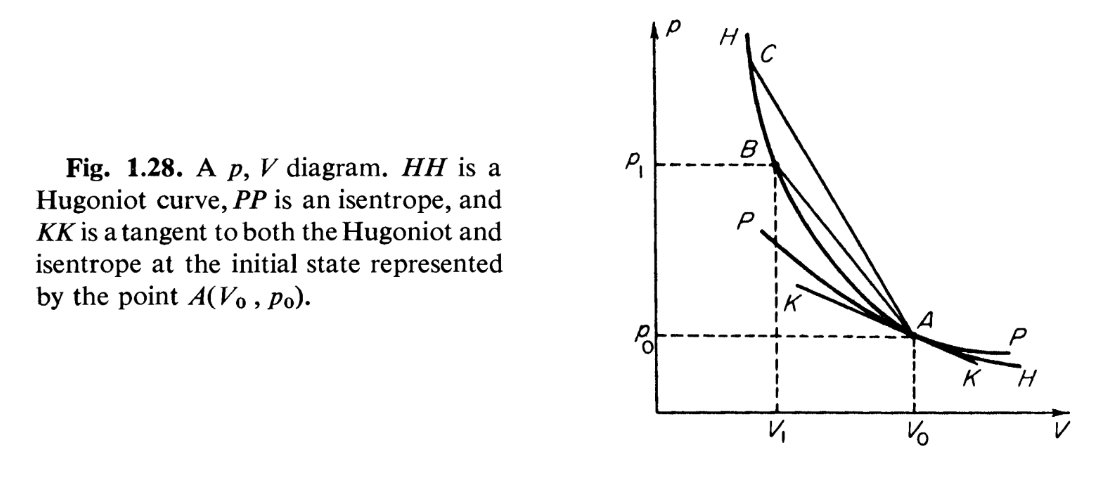
\includegraphics[width=1\textwidth]{figures/fig_1_28.png} 
  \end{center}
  \item Both the Hugoniot and Isentrope curves are convex downwards, and they are tangent at point A (proper calculation ahead).
  \item One notices that another point B($p_1, V_1$) symbolizes another state that can be achieved through a shock wave from state A, and the point P($p_1, V_2$) symbolizes the state that can be achieved through an isentropic process from state A.
  \item From the velocity equation \ref{u_shock} (Eq. 1.67 in the book), one can write the shock speed squared as the negative of slope of the secant line AB:
  \begin{equation}
    D^2 = u_0^2 = -V_0^2  \frac{(p_1 - p_0)}{V_1 - V_0}
  \end{equation}
  this formula shows explicitly that the higher final pressure $p_1$ $\to$ the higher shock speed $D$.
  \item Using Eq. (1.75) in the book (which is the ratio of specific volumes across the shock), one can calculate the derivative of the curve:
  \begin{align}
      \frac{dp_1}{dV_1} &= \frac{d}{dV_1} \left[ \frac{(\gamma + 1)V_0 - (\gamma - 1)V_1}{(\gamma + 1)V_1 - (\gamma - 1)V_0} p_0 \right] \\
      &= -\frac{(\gamma - 1)p_0}{(\gamma + 1)V_1 - (\gamma - 1)V_0} - \frac{(\gamma + 1)V_0 - (\gamma - 1)V_1}{\left[ (\gamma + 1)V_1 - (\gamma - 1)V_0 \right]^2} (\gamma + 1) p_0
    \end{align}
  By setting $V_1 = V_0$ in the above equation, one gets the slope of the Hugoniot curve at point A:
  \begin{equation}
    \left( \frac{dp}{dV} \right)_{Hugoniot, A} = -\frac{\gamma p_0}{V_0}
  \end{equation}
  which is exactly the slope of the isentrope curve at point A ($PV^\gamma \sim const \Rightarrow \left(\frac{\partial p}{\partial V}\right)_S = -\frac{\gamma p}{V}wg7$)
  \item One can notice that the shock velocity under the limit of weak shocks ($p_1 \approx p_0$) is:
  \begin{equation}
    D^2 = -V_0^2 \frac{p_1-p_0}{V_1 - V_0} \to \left( \frac{dp}{dV} \right)_{Hugoniot, A} = \gamma p_0 V_0 = c_0^2
  \end{equation}
  and also $D=u_0 > c_0$ (supersonic flow into the shock) as expected since the curve is convex downwards. It means that the initial slope of the Hugoniot curve at point A is defined by the speed of sound in the gas.
  \item In section 1.18 we will show that also the second derivative of the Hugoniot and Isentrope curves are equal at point A, which means that the two curves are \textbf{tangent up to second order at point A}.
  \end{enumerate}
  \subsection{The difference between the shock and isentropic processes as a change in entropy}
  \begin{enumerate}
    \item One should notice that the change in the specific energy during the shock compression form state A to state B is:
    \begin{equation}
      \Delta \varepsilon_{AB} = \varepsilon_1 - \varepsilon_0 = \frac{1}{2} (p_1 + p_0)(V_0 - V_1)
    \end{equation}
    according to Eq. \ref{Hugoniot Energy} (Eq. 1.71 in the book). This is exactly the area of the trapezoid MABN in fig. 1.29 in the book. 
    \begin{center}
      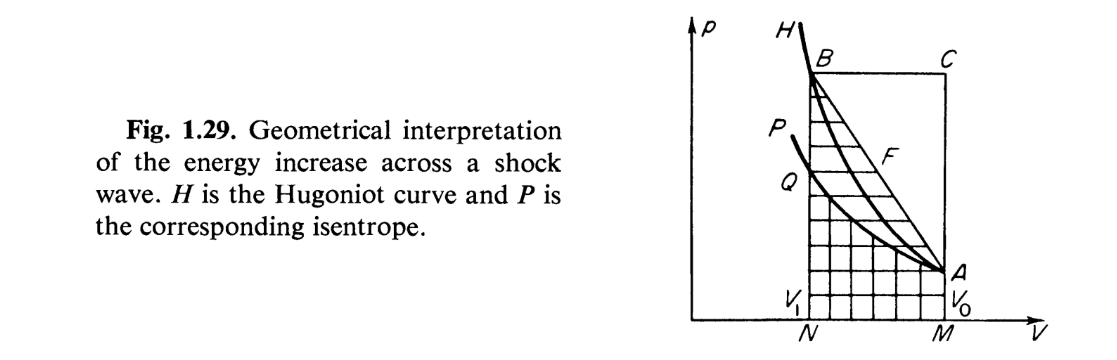
\includegraphics[width=1\textwidth]{figures/fig_1_29.png}
    \end{center}
    \item One can imagine an isentropic process from state A to state P, followed by a heating process from state P to state B (vertical line, isochoric processes). The total energy change in this process is:
    \begin{equation}
      \Delta \varepsilon_{APB} = \int_{S_0}^{S_1} T dS = \varepsilon_1 - \varepsilon^\prime
    \end{equation}
    where we sticked here to the book's notation where $\varepsilon^\prime$ is the specific energy at point P.
    \item Another cool property is the area of the rectangle MNBC, which is equal to $p_1 (V_0 - V_1)$ which is exactly the total work done on a unit mass of gas during the piston compression from state A to state B. Across a strong shock when $p_1 \gg p_0$, the area of the rectangle is approximately twice the area of the trapezoid, which means that half of the work done on the gas is converted to an increase in internal energy, while the other half is dissipated as an increase in entropy. One can see that from the change in kinetic energy per unit mass across the shock:
    \begin{equation}
      \frac{u^2}{2} = \frac{(u_0 - u_1)^2}{2} = \frac{1} {2} \left( \frac{p_1 - p_0}{V_0 - V_1} \right) \to \frac{1}{2}p_1 (V_1 - V_0) \quad \text{for } p_1 \gg p_0
    \end{equation}
  \end{enumerate}  
  \subsection{Two successive shocks}
  \begin{enumerate}
    \item Suppose that the gas is initially at state A($p_0, V_0$), then it is compressed through a shock wave to state B($p_1, V_1$) on $H_A$ curve, and then it is compressed again through another shock wave to another point in the illustrated $H_B$. This is shown in fig. 1.30 in the book.
    \begin{center}
      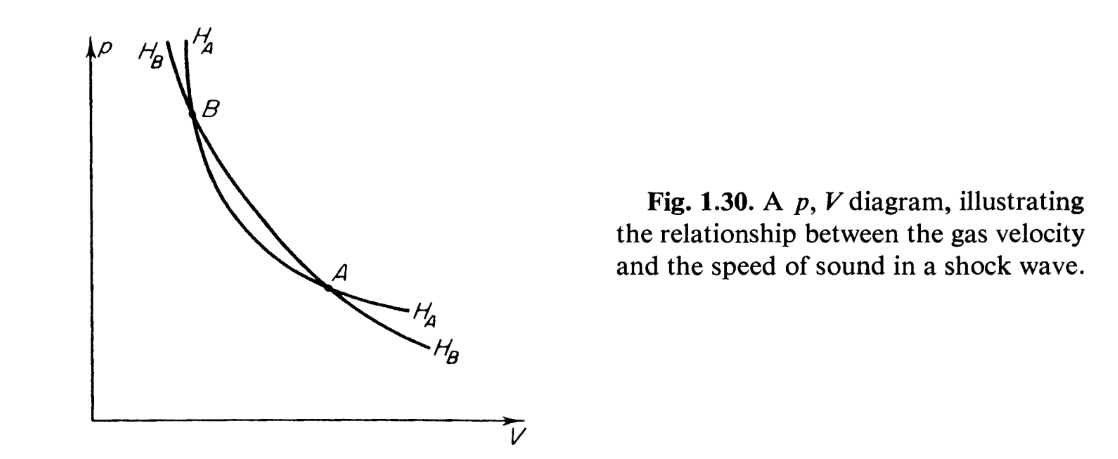
\includegraphics[width=1\textwidth]{figures/fig_1_30.png}
    \end{center}
    Since the Hugoniot function $p_1 = H(V_1; p_0, V_0)$ is symmetric to the permutation 1 $\leftrightarrow$ 0 (can be seen from Eq. \ref{Hugoniot}), the point A also lies on the Hugoniot curve $H_B$. 
    \item Another interesting point that arises from this graph is the fact that $u_1 < c_1$ (subsonic flow out of the shock). It is seen from these equations:
    \begin{align}
      u_1^2 &= -V_1^2 \frac{p_1 - p_0}{V_1 - V_0} \\
      c_1^2 &= -V_1^2 \left( \frac{\partial p}{\partial V} \right)_{H_B, S}
    \end{align}
    and it is seen from the graph that the slope of the tangent line at point B is steeper than the slope of the secant line AB, which means that $u_1^2 < c_1^2$ or $M_1 < 1$ as expected.
    \item The book also comments about the physical reason for the feature that $H_B$ passes to the left of $H_A$ at pressures higher than $p_1$. It says that since the volume in a shock compression is bounded by $V_B > \frac{\gamma - 1}{\gamma + 1} V_A$, the second shock can decrease the volume to a state C with a lower boundary which is $V_C > \frac{\gamma - 1}{\gamma + 1} V_B > \left( \frac{\gamma - 1}{\gamma + 1} \right)^2 V_A$.
    \item At the top of pg. 59, the book comments that it's impossible to reach a final state $(p_1, V_1)$ through two successive shocks that is different from the state achieved through a single shock from the initial state $(p_0, V_0)$. This process is shown in fig. 1.31 in the book.
    \begin{center}
      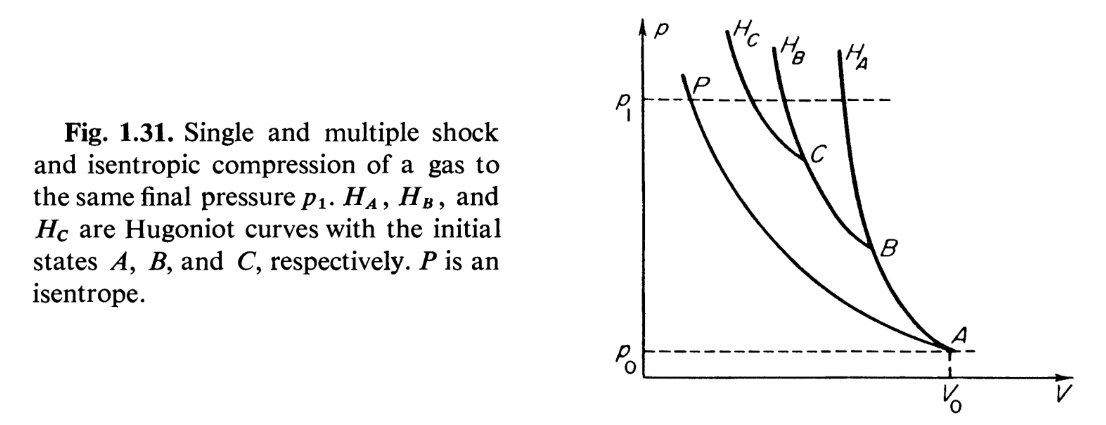
\includegraphics[width=1\textwidth]{figures/fig_1_31.png}
    \end{center}
    The book also says that this fact can be proven using the fact that the Hugoniot curves are function of two parameters $(p_0, V_0)$ and \textcolor{red}{I need to understand why (optional though)}.
  \end{enumerate}
  \section{On the impossibility of a rarefaction shock wave in a normal fluid}
  \subsection{Analysis using the second law of thermodynamics}
  \begin{enumerate}
    \item Inequalities (1.86) \& (1.87) in the book show the difference in the discontinuity relations between shock waves and rarefaction shocks. For shock waves - $p_1, \rho_1, S_1 > p_0, \rho_0, S_0$ while for rarefaction shocks - $p_1, \rho_1, S_1 < p_0, \rho_0, S_0$.
    This is shown by Fig. 1.32 in the book.
    \begin{center}
      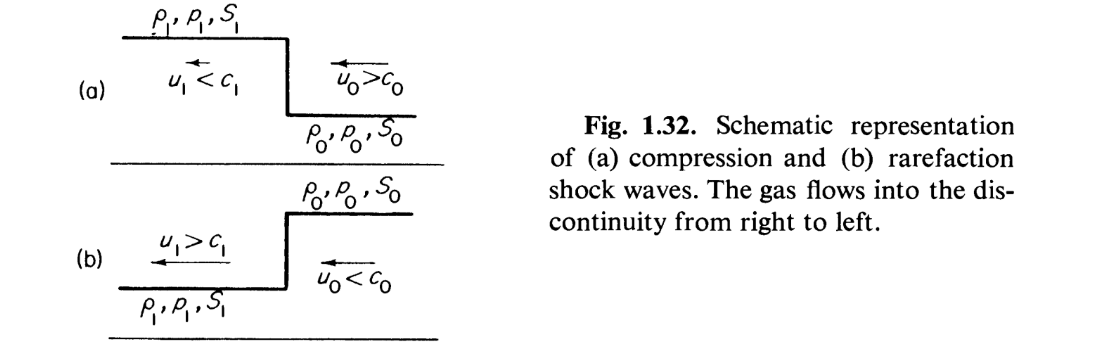
\includegraphics[width=1\textwidth]{figures/fig_1_32.png}
    \end{center}
    The book emphasizes the fact that the conservation laws themselves \textbf{do not forbid the existence of rarefaction shocks}, but rather the second law of thermodynamics (the increase in entropy) forbids their existence in normal fluids - the explanation is given through the analysis of fig. 1.33 where the final state B lies on the right side (bigger volume) of the initial state A on the Hugoniot curve, which means that $S_1 < S_0$, e.g. a decrease in entropy.
    \begin{center}
      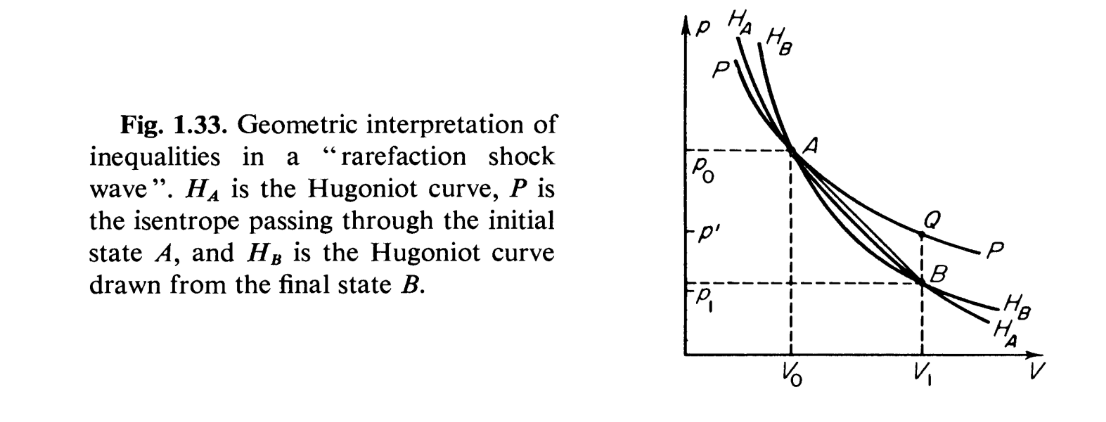
\includegraphics[width=1\textwidth]{figures/fig_1_33.png}
    \end{center}
    \item The book says that this phenomenon is general and applies to all fluids where the Hugoniot curves are convex downwards in the $p-V$ plane, e.g. $\left( \frac{\partial^2 p}{\partial V^2} \right)_H > 0$ (these are called "normal fluids"), and it says that this statement will be proven for weak shockwaves in section 1.18.
  \end{enumerate}
  \subsection{Explanation using Mechanical Stability}
  \begin{enumerate}
    \item The book discusses (pg. 61-62) the mechanical stability argument that explains the impossibility of rarefaction shocks in normal fluids.
    \item It says (mid pg. 62) that a wave that propagates through a fluid supersonically is "stable" in the sense that small perturbations ahead of the wave cannot affect the wave structure, while a wave that propagates subsonically is "influencable" in the sense that small perturbations ahead of the wave can affect the wave structure.
    \item Therefore, a shock wave is stable regarding small perturbations that occur behind the shock front (because it propagates through the undisturbed gas in a supersonic speed), while it's strength \textbf{is} influencable by small perturbations that occur behind it since it propagates through the disturbed gas in a subsonic speed (which explains the fact that heating/cooling or compressing/expanding the gas behind the shock can affect its strength).
    This means that strength is influencable in a shock wave, but the wave structure is stable.
    \item On the other hand, the strength of a rarefaction shock is stable (since it propagates through the undisturbed gas in a supersonic speed), but its structure is influencable (since it propagates through the disturbed gas in a subsonic speed). This means that the rarefaction shock structure is not stable as a discontinuity, and it's also not physical.
    \end{enumerate}
  \subsection{On the relation between entropy to stability}
    The book actually showed the significant result that can be summarized using the following relation by ChatGPT:
    \begin{equation}
      \text{Entropy Increase} \iff \text{Causal Control of the Shock} \iff \text{Wave Structure Stability}
    \end{equation}
    This conclusion is also spectacularly summarized in table 1.1 in the book, that relates it to the section of the book where it is discussed rarefaction smooth waves (section 1.12) and centered compression simple waves (section 1.13).
    \begin{center}
      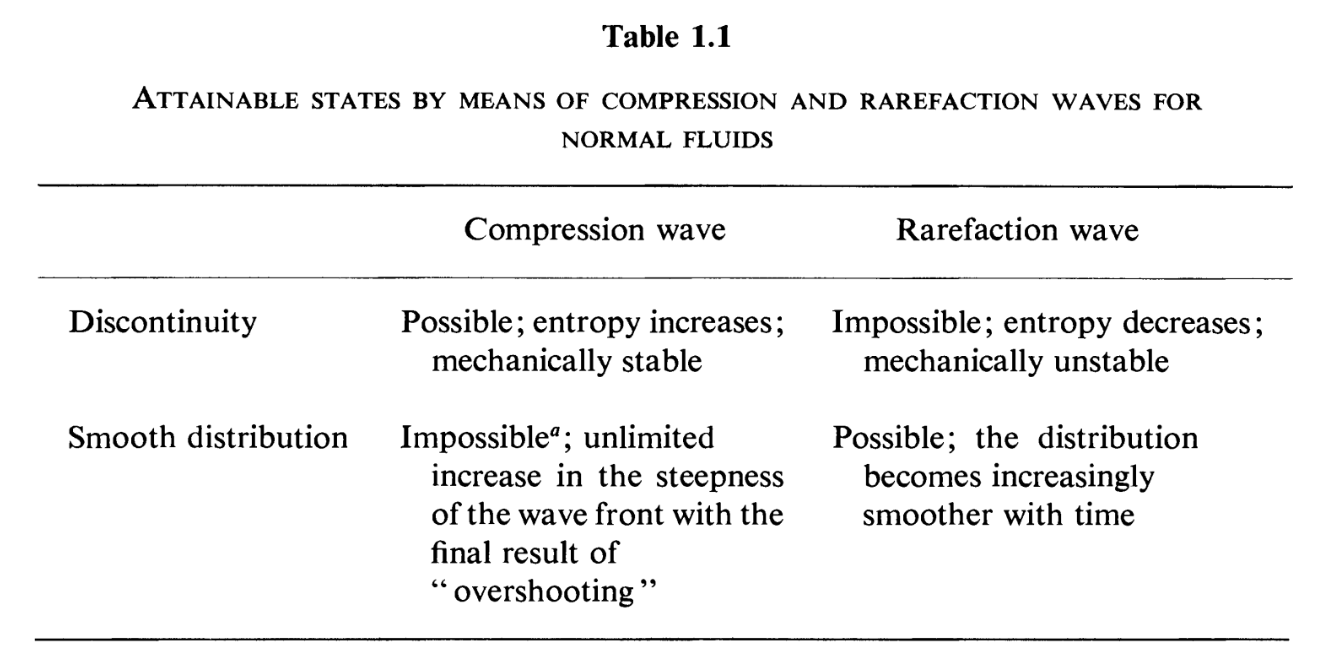
\includegraphics[width=1\textwidth]{figures/table_1_1.png}
    \end{center}
    \section{Weak shock waves}
    \subsection{Derivation of the impossibility of a rarefaction shock wave for a weak shock in a general normal gas}
    \begin{enumerate}
      \item The book asssumes now a general gas (with a general function $\varepsilon(S, V)$) and analyzes weak shocks where $\varepsilon_1-\varepsilon_0$ is small so the Hugoniot curve can be expanded in Taylor series around point A($p_0, V_0$):
      \item The theoretical equation for a Hugoniot curve is:
      \begin{equation}
        \varepsilon_1 - \varepsilon_0 = \frac{1}{2} (p_1 + p_0)(V_0 - V_1)
      \end{equation}
      The Taylor expansion of the LHS around point A (for 1st order in $\Delta S$ and 3rd order in $\Delta V$) is:
      \begin{equation}
        \varepsilon_1 - \varepsilon_0 = \left(\frac{\partial \varepsilon}{\partial S}\right)_V (S_1 - S_0) + \left( \frac{\partial \varepsilon}{\partial V} \right)_S (V_1 - V_0) + \frac{1}{2} \left( \frac{\partial^2 \varepsilon}{\partial V^2} \right)_S (V_1 - V_0)^2 + \frac{1}{6} \left( \frac{\partial^3 \varepsilon}{\partial V^3} \right)_S (V_1 - V_0)^3 + ...
      \end{equation}
      which according to the thermodynamic relation $d\varepsilon = T dS - p dV$ can be written as:
      \begin{equation}
        \varepsilon_1 - \varepsilon_0 = T_0(S_1-S_0) -p_0 (V_1 - V_0) - \frac{1}{2} \left( \frac{\partial p}{\partial V} \right)_S (V_1 - V_0)^2 - \frac{1}{6} \left( \frac{\partial^2 p}{\partial V^2} \right)_S (V_1 - V_0)^3 + ...
      \end{equation}
      The RHS can be expanded as (to the same orders as):
      \begin{equation}
        \frac{1}{2} (p_1 + p_0)(V_0 - V_1) = \left( \frac{\partial p}{\partial S} \right)_V (S_1 - S_0)(V_0 - V_1) - p_0 (V_1- V_0) - \frac{1}{2} \left( \frac{\partial p}{\partial V} \right)_S (V_1 - V_0)^2 - \frac{1}{4} \left( \frac{\partial^2 p}{\partial V^2} \right)_S (V_1 - V_0)^3 + ...
      \end{equation}
      If we neglect the term $\left( \frac{\partial p}{\partial S} \right)_V (S_1 - S_0)(V_0 - V_1)$ under the argument that $\Delta S \sim \Delta V^3$ (which will be consistent with the final result), we can equate the two expansions to get:
      \begin{equation}
        T_0 (S_1 - S_0) = \frac{1}{12} \left( \frac{\partial^2 p}{\partial V^2} \right)_S (V_1 - V_0)^3
      \end{equation}
      which finally shows that with normal gases (with $\left( \frac{\partial^2 p}{\partial V^2} \right)_S > 0$) the entropy increases across a weak shock wave ($S_1 > S_0$), while rarefaction shocks ($V_1 > V_0$) are impossible since they would cause a decrease in entropy ($S_1 < S_0$). More explanation about it (\textcolor{red}{Including the neuances about what the definition of a "normal" gas actually means and how it relates to the coefficient of thermal expansion at constant pressure}) is given at the bottom of pg. 64.
    \end{enumerate}
    \subsection{Relation between the expansion of the Hugoniot and Isentrope curves at point A}
    \begin{enumerate}
      \item One can expand the pressure along the isentrope \& Hugoniot curves around point A in Taylor series up to third order in $\Delta V$:
      \begin{align}
        p_{Isentrope} &= p_0 + \left( \frac{\partial p}{\partial V} \right)_S (V_1 - V_0) + \frac{1}{2} \left( \frac{\partial^2 p}{\partial V^2} \right)_S (V_1 - V_0)^2 + \frac{1}{6} \left( \frac{\partial^3 p}{\partial V^3} \right)_S (V_1 - V_0)^3 + ... \\
        p_{Hugoniot} &= p_0 + \left( \frac{\partial p}{\partial V} \right)_S (V_1 - V_0) + \frac{1}{2} \left( \frac{\partial^2 p}{\partial V^2} \right)_S (V_1 - V_0)^2 + \frac{1}{6} \left( \frac{\partial^3 p}{\partial V^3} \right)_S (V_1 - V_0)^3 + ...
      \end{align}
      where the third-order term in the Hugoniot expansion includes the linear term in $\Delta S$ as should be considered from the previous section.
      \textcolor{red}{Need to FIX!!!! And understand BTW}
      \item That being said, one can see that the first and second derivatives of the Hugoniot and Isentrope curves are equal at point A, while the third derivatives are different by the term:
      \begin{equation}
        \left( \frac{\partial p}{\partial S} \right)_{V} (S_1 - S_0) = -\frac{1}{12T_0} \left( \frac{\partial p}{\partial S} \right)_V \left( \frac{\partial^2 p}{\partial V^2} \right)_S (V_1 - V_0)^3 
      \end{equation}
      and since the terms $\left( \frac{\partial p}{\partial S} \right)_V > 0$ and $\left( \frac{\partial^2 p}{\partial V^2} \right)_S > 0$ for normal gases, the third derivative of the Hugoniot curve is less than the third derivative of the Isentrope curve at point A - which means that the Hugoniot curve passes below the Isentrope curve for $V_1 > V_0$ as shown in fig. 1.34.
      \begin{center}
        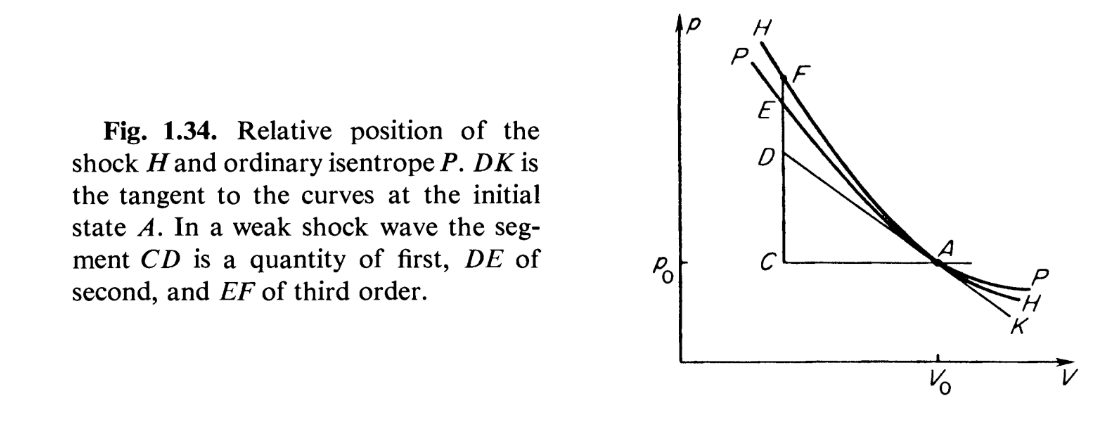
\includegraphics[width=1\textwidth]{figures/fig_1_34.png}
      \end{center}
      \textcolor{blue}{This proof should also be validated in my understanding.}
    \end{enumerate}
    \subsection{Geometric interpretation of the arguments}
    \begin{enumerate}
      \item The book discusses (pg. 66 bottom - 67) the geometric interpretation of the arguments above using fig. 1.35 in the book.
      \begin{center}
        % \includegraphics[width=1\textwidth]{figures/fig_1_35.png}
        % TODO: Add fig_1_35.png to the figures folder
      \end{center}
      The book says that the correction for the area of the triangle ABC to the entire area ABCEA which is equal $\bar{T}\Delta S$ (where $\bar{T}$ is some average temperature between $T_0$ and $T_1$) is of a higher order (i.e. $\Delta V^4$) and therefore negligible for weak shocks.
      It suggests that one can see geometrically through expressing the area of ABCEA as:
      \begin{equation}
        \text{Area} = \bar{T}\Delta S = \frac{p_0 + p_1}{2}(V_0 - V_1) - \int_{V_1}^{V_0} P(V, S_0) dV
      \end{equation}
      which is exactly the area of the trapezoid MABN (M,N don't appear in this figure so imagine them on the vertical lines from A and B to the V axis) minus the area under the isentrope curve from $V_1$ to $V_0$.
      
      Then, the book says to substitute the third-order expansion for $p$ along the isentrope curve to get the same relation (1.88) in the book.
      \textcolor{red}{I asked chatGPT to do so, it might be a wonderful exercise to practice the Taylor expansions...}

      \item The book also compares the slopes of the secant line AB and the tangent line at points A,B. It does so by expanding these slopes to the first order in $\Delta V$:
      \begin{align}
        \frac{p_1 - p_0}{V_1 - V_0} &= \left( \frac{\partial p}{\partial V} \right)_S + \frac{1}{2} \left( \frac{\partial^2 p}{\partial V^2} \right)_S (V_1 - V_0) + O(\Delta V^2) \\
        \left( \frac{\partial p}{\partial V} \right)_{S_A} &= \left( \frac{\partial p}{\partial V} \right)_{S_0} \\ 
        \left( \frac{\partial p}{\partial V} \right)_{S_B} &= \left( \frac{\partial p}{\partial V} \right)_{S_0} + \left( \frac{\partial^2 p}{\partial V^2} \right)_S (V_1 - V_0) + O(\Delta V^2)
      \end{align}
      where the tangent slope at point B was expanded using the expansion of the derivative $\left( \frac{\partial p}{\partial V} \right)_S$ along the isentrope curve around point A (where $S=S_0$). \textcolor{red}{I need to understand this point better.}

      \textcolor{blue}{\textbf{A very important quote of the book regarding to the deepness of the geometric interpretations:}}: "Of importance is the inner connection between the condition for entropy increase and that for mechanical stability of the discontinuity $u_0 > c_0$. \underline{(The geometric interpretation) Both conditions follow directly from the (convexity of the Hugoniot curve in the $p-V$ plane) fact that the slope of the isentropic and Hugoniot curves increase with decreasing volume.}"
    \subsection{Summary - The proven properties of weak shocks in normal fluids}
    The following are the actual properties that were proven about weak shocks in normal fluids (in which $\left( \frac{\partial^2 p}{\partial V^2} \right)_S > 0$):
    \begin{enumerate}
      \item For a shock wave the entropy increases through the shock - $S_1 > S_0$ while for a rarefaction shock the entropy decreases through the shock - $S_1 < S_0$ (pg. 63-64 analytically and pg. 65 bottom - 66 topgeometrically). The entropy increase is proportional to the cube of the volume difference across the shock - $\Delta S \sim (V_1 - V_0)^3$ (e.g. very small for weak shocks).
      
      \item The Hugoniot and Isentrope curves are tangent up to second order at point A (pg. 64 bottom -65 top).
      \item 
      \item For shock wave $u_0 > c_0$ (supersonic flow into the shock) \& $u_1 < c_1$ (subsonic flow out of the shock) - and the other way around for rarefaction shocks (pg. 66 bottom - pg. 67 top geometrically). 
    \end{enumerate}
    \end{enumerate}
    \section{Shock waves in a fluid with anomalous thermodynamic properties}
    This section is divided into two subsections:
    \begin{enumerate}
      \item Analyzing gases for which the condition for normal fluids is violated - e.g. their isentropes and Hugoniot curves are convex upwards in the $p-V$ plane. For these gases, rarefaction shocks are possible while compression shocks are impossible (for the reasons of entropy increase and mechanical stability explained before). 
      \item An example of such fluids are liquids near the critical point, where the coefficient of thermal expansion at constant pressure is negative - this is shown in fig. 1.37 and explained in the bottom of pg. 68 and slightly before the section ends.
      \begin{center}
        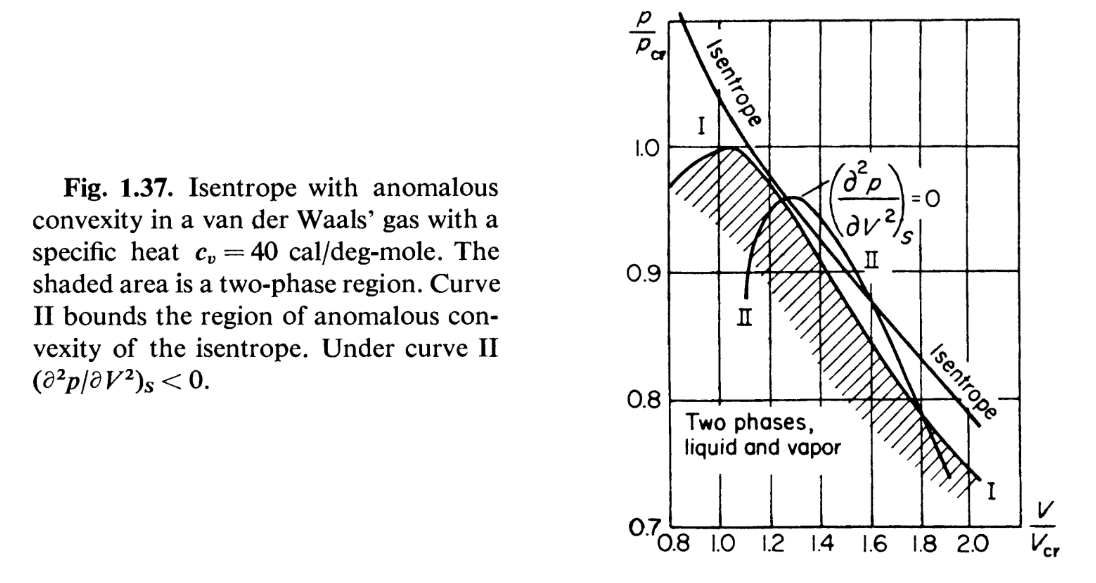
\includegraphics[width=1\textwidth]{figures/fig_1_37.png}
      \end{center}
    \end{enumerate}
\section{Equations of 1D gas flow}
\subsection{Introduction}
\begin{enumerate}
  \item The book introduces the fact that dissipative processes are viscosity and heat conduction, and are both neglected in the Euler equations. These processes lead to \textbf{nonadiabatic and thermodynamically irreversible} phenomena in the gas flow, and they appear only when there are large gradients in the flow variables (like in shock waves).
  \item The book says that we are going to deal with only the 1D planar solution.
\end{enumerate}
\subsection{Considering viscosity - derivation of the generalized momentun tensor}
\begin{enumerate}
  \item The book presents a cross section of the flow surrounded by two adjacent layers whose thickness is of the order of the mean free path $l$ (fig. 1.38 in the book) - in the volumes of these layers, the particles are asssumed to have a constant velocity $u$ (since we suppose that a change in velocity happens through collision, which happens for each molecule only after traveling a distance of the order of $l$).
  \begin{center}
      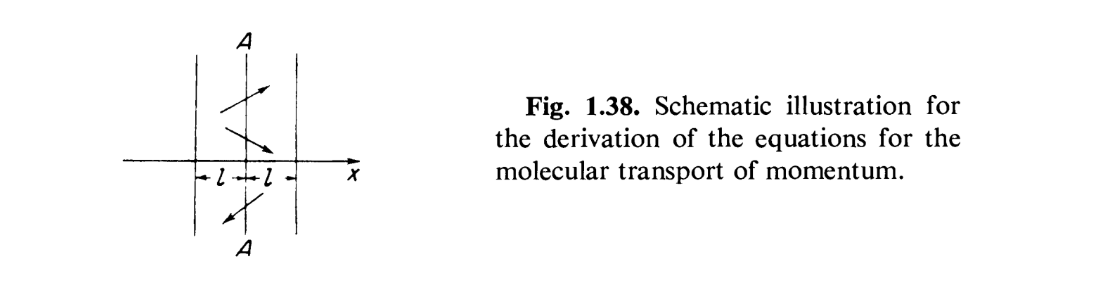
\includegraphics[width=1\textwidth]{figures/fig_1_38.png}
  \end{center}
  \item Then, the book analyzes the amount of pressure that is exerted on the cross section by the particles in the two layers. It turns out that this pressure equals to the rate of momentum transfer per unit area from the two layers to the cross section. For that we define $m$ as the mass of each particle, $n$ as the number density of particles, and $\nu$ as the average velocity of particles in each layer (which is of the order of the thermal velocity). The rate of momentum transfer from the left layer to the cross section is:
  \begin{equation}
    \text{Rate of momentum transfer from left layer} = n\nu\cdot m u
  \end{equation}
  while the rate of momentum transfer from the right layer to the cross section is:
  \begin{equation}
    \text{Rate of momentum transfer from right layer} = -n\nu \cdot m (u + \Delta u) = -n\nu \cdot m u - n\nu \cdot m l \frac{\partial u}{\partial x}
  \end{equation}
  Therefore, the total rate of momentum transfer to the cross section per unit area and unit time is:
  \begin{equation}
    \text{Total rate of momentum transfer} = - n \nu m l \frac{\partial u}{\partial x}
  \end{equation}
  Therefore, the viscous stress (the extra pressure due to viscosity) is:
  \begin{equation}
    \tau_{xx} = -\sigma' = - \frac{4}{3}\mu \frac{\partial u}{\partial x}
  \end{equation}
  where $\frac{4}{3}$ is a numerical factor that comes from a more accurate kinetic theory calculation for an ideal gas, and $\mu \propto n m \nu l = \rho \nu l$ is the dynamic viscosity coefficient of the gas.
  \textcolor{blue}{The chatGPT says that viscosity is rate of momentum diffusion that arises from the velocity gradients in the fluid, which physically means that particles from faster layers transfer momentum to slower layers through collisions, which is exactly what we analyzed here. In contrast, thermodynamic pressure arises from the random isotropic motion of particle that exists even in the a unifrom flow without velocity gradients (e.g. equillibrium).}
  \item Therefore, the generalized momentum flux tensor that includes the effect of viscosity is:
  \begin{equation}
    \Pi_{xx} = p - \sigma' = p - \frac{4}{3} \mu \frac{\partial u}{\partial x}
  \end{equation}
  and the continuity equation is:
  \begin{align}
    \frac{\partial}{\partial t}(\rho u) = -\frac{\partial \Pi_{xx}}{\partial x} \\
    \rho \frac{Du}{Dt} = -\frac{\partial}{\partial x}(p - \sigma')
  \end{align}
  and the book says that $\frac{\partial \sigma}{\partial x}$ is the viscous (e.g. internal friction) force per unit volume that acts to reduce velocity gradients in the fluid.
  \end{enumerate}

  \subsection{Considering Heat conduction - generalized energy flux}
  \begin{enumerate}
    \item The effective decrement in momentum flux due to viscosity leads to a decrease in the kinetic energy of the fluid, which is converted to internal energy (heating) through viscous dissipation. Therefore, a term of $\sigma'u$ analogous to $pu$ should be added to the energy flux.
    \item The energy flux per unit area and unit time due to heat conduction is given by Fourier's law:
    \begin{equation}
      J = -\kappa \frac{\partial T}{\partial x}
    \end{equation}
    where $\kappa$ is the thermal conductivity of the gas and is of the order of $\rho c_p \nu l$.
    \item Therefore, the generalized energy flux that includes the effects of viscosity and heat conduction is:
    \begin{equation}
      \frac{\partial}{\partial t} \left[ \rho \left( \varepsilon + \frac{u^2}{2} \right) \right] = -\frac{\partial}{\partial x} \left[ \rho u \left( \varepsilon + \frac{u^2}{2} \right) + (p - \sigma')u - \kappa \frac{\partial T}{\partial x} \right]
    \end{equation}
    which can be transformed with the aid of the continuity \& momentum equations (and also the second law of thermodynamics) to the following equation:
    \begin{equation}
      \rho T \frac{DS}{Dt} = \sigma' \frac{\partial u}{\partial x} - \frac{\partial J}{\partial x} = \frac{4}{3} \mu \left( \frac{\partial u}{\partial x} \right)^2 + \frac{\partial}{\partial x} \left( \kappa \frac{\partial T}{\partial x} \right)
    \end{equation}
    The book comments that the viscosity term is always positive and represents the irreversible conversion of kinetic energy to internal energy (heating) due to viscous dissipation, while the heat conduction term can be positive or negative depending on the temperature gradient.
    \item Dispite the last comment, the book emphasizes that both viscosity and heat conduction lead to an increase in entropy in the fluid (e.g. irreversible processes) as should be expected from the second law of thermodynamics. This can be seen through the integration of the heat conduction term over a volume bounded by two surfaces at $x=x_1<x_2$ - which leads to a positive contribution to the total entropy change in the volume.
    \end{enumerate}
  \subsection{Definition of Reynolds \& Peclet numbers}
  \begin{enumerate}
    \item These two dimensionless numbers are defined in order to compare the relative importance of the dissipative processes (viscosity and heat conduction) to the advective transport of momentum and energy in the fluid.
    \item If we suppose that $U$ is the characteristic velocity \& $d$ is the characteristic length scale of the flow region - we can claim that:
    \begin{align}
      \varepsilon_{\text{advection}} &= \rho u \frac{\partial u}{\partial x} \sim \frac{\rho U^2}{d} \\
      \varepsilon_{\text{viscosity}} &= \frac{\partial\sigma'}{\partial x} = \frac{4}{3} \mu \frac{\partial^2 u}{\partial x^2} \sim \frac{\mu U}{d^2} \\
      \varepsilon_{\text{heat conduction}} &= \frac{\partial J}{\partial x} = \frac{\partial}{\partial x} \left( -\kappa \frac{\partial T}{\partial x} \right) \sim \frac{\kappa \Delta T}{d^2} \sim \frac{\kappa U}{c_p d^2}
    \end{align}
    The Reynolds and Peclet numbers are defined as the ratios of advective transport to dissipative transport:
    \begin{align}
      Re &= \frac{\varepsilon_{\text{advection}}}{\varepsilon_{\text{viscosity}}} = \frac{\rho U^2 / d}{\mu U / d^2} = \frac{\rho U d}{\mu} = \frac{\nu}{U d}\\
      Pe &= \frac{\varepsilon_{\text{advection}}}{\varepsilon_{\text{heat conduction}}} = \frac{\rho U^2 / d}{\kappa U / c_p d^2} = \frac{\rho c_p U d}{\kappa} = \frac{\chi}{U d}
    \end{align}
    where $\nu = \frac{\mu}{\rho}$ is the kinematic viscosity and $\chi = \frac{\kappa}{\rho c_p}$ is the thermal diffusivity of the gas.
    \item The book comments that $\chi,\nu\sim \nu l$ by definition (they differ by a proportionality constant of order unity). Therefore, the Reynolds and Peclet numbers are of the same order of magnitude. 
    \item In flows where $Re, Pe \gg 1$, the dissipative processes are negligible compared to the advective transport of momentum and energy. However, in regions with large gradients in the flow variables (like shock waves), the dissipative processes become significant even if $Re, Pe \gg 1$ globally because the characteristic length scale $
    frac{d}{l}$ becomes very small in these regions.
  \end{enumerate}
  

\end{document}